%%%%%%%%%%%%%%%%%%%%%%%%%%%%%%%%%%%%%%%%%
% OIST Doctoral Thesis - Final bound version
% LaTeX Template
% Version 0.2 (2016/04/06)
%
% This version is the final binding version which will be published.
%
% Original author:
% Jeremie Gillet
%
%%%%%%%%%%%%%%%%%%%%%%%%%%%%%%%%%%%%%%%%%

%----------------------------------------------------------------------------------------
%	PACKAGES AND OTHER DOCUMENT CONFIGURATIONS
%----------------------------------------------------------------------------------------

\documentclass[12pt, twoside]{book} % 12 pt font, two-sided book style
\usepackage[a4paper, includehead, headheight=0.6cm, inner=3cm ,outer=2.5cm, top=2.5 cm, bottom=2.5cm]{geometry}  % Changing size of document
\usepackage[english]{babel} % The document is in English
\usepackage[utf8]{inputenc} % UTF8 encoding
\usepackage[T1]{fontenc} % Font encoding

\usepackage{graphicx} % For including images

\usepackage{longtable} % tables that can span several pages
\usepackage[bf]{caption} % caption: FIG in bold
\usepackage{fancyhdr} % For the headers
\newcommand{\softmax}{\textit{softmax}}
\newcommand{\maximize}{\textit{maximize}}

\usepackage{amsmath}
\usepackage[linesnumbered,ruled,algo2e]{algorithm2e}
\usepackage{amsfonts}
\setlength{\headheight}{28pt}

\newcommand{\kechen}[1]{\textcolor{red}{[Kechen]: {#1}}}



\newcommand{\numberedchapter}{ % Preparation for numbered chapters
	\cleardoublepage % To make sure the previous headers are passed
	\fancyhead[RE]{{\bfseries \leftmark}}% Headers for left pages
	\fancyhead[LO]{{\bfseries \rightmark}}}% Headers for right pages
\newcommand{\unnumberedchapter}[1]{ % Preparation for unnumbered chapters
	\cleardoublepage % To make sure the previous headers are passed
	\addcontentsline{toc}{chapter}{#1} % Also adds the chapter name to the Contents
	\fancyhead[RE]{{\bfseries #1}} % Headers for left pages
	\fancyhead[LO]{}}%Headers for right pages

\usepackage{emptypage} % No headers on an empty page

% \usepackage{eso-pic} % For the background picture on the title page
% \newcommand\BackgroundPic{%
% \put(-170,-160){%
% \parbox[b][\paperheight]{\paperwidth}{%
% \vfill
% \centering
% \includegraphics[width=0.5\paperwidth]{symbol.png}%
% \vfill
% }}}

\usepackage{hyperref} % Adds clickable links at references

%----------------------------------------------------------------------------------------
%	ADD YOUR CUSTOM VALUES, COMMANDS AND PACKAGES
%----------------------------------------------------------------------------------------

% Open Preamble/mydefinitions.tex and enter some values (name, thesis title...) 
% and include your own custom LaTeX functions and packages

%----------------------------------------------------------------------------------------
%	VALUES FOR THE THESIS
%----------------------------------------------------------------------------------------

\newcommand{\name}{\href{http://www.ccis.neu.edu/home/kechenqin/}{Kechen Qin}} % Author name
\newcommand{\thesistitle}{Machine Learning for Text using Latent Information} % Title of the thesis
\newcommand{\submissiondate}{April, 2020} % Submission date "Month, year"
\newcommand{\supervisor}{\href{https://www.khoury.northeastern.edu/people/jay-javed-aslam/}{Javed A. Aslam}} % Supervisor name
\newcommand{\committee}{\href{https://www.khoury.northeastern.edu/people/jay-javed-aslam/}{Javed A. Aslam}} % Co-Supervisor name, comment this line if there is none
\newcommand{\committeemore}{\href{https://www.khoury.northeastern.edu/people/virgil-pavlu/}{Virgil Pavlu}}
\newcommand{\committeemoreII}{\href{https://www.khoury.northeastern.edu/people/chris-amato/}{Christopher Amato}}
\newcommand{\committeemoreIII}{\href{https://ieeexplore.ieee.org/author/37269034000}{Xiaohui Cui}}



%----------------------------------------------------------------------------------------
%	BIBLIOGRAPHY STYLE (pick the style you want)
%----------------------------------------------------------------------------------------

\usepackage[square, numbers, sort&compress]{natbib} % for bibliography - Square brackets, citing references with numbers, citations sorted by appearance in the text and compressed (as in [4-7])
%\usepackage[longnamesfirst,round]{natbib} % Natural Sciences bibliography

\bibliographystyle{Preamble/physics_bibstyle} % You may use a different style adapted to your field
%\bibliographystyle{unsrtnat} % You may use a different style adapted to your field


%----------------------------------------------------------------------------------------
%	YOUR PACKAGES (be careful of package interaction)
%----------------------------------------------------------------------------------------

\usepackage{amsthm,amsmath,amssymb,amsfonts,bbm}% Math symbols
\usepackage{amsbsy,bm}
\usepackage{float}
\usepackage{times}
\usepackage{latexsym}
\usepackage{csvsimple}
\usepackage{url}
\usepackage{graphicx}  %Required
\usepackage{subfigure}
\usepackage{multirow}
\usepackage{xcolor}
\usepackage{algorithm}
\usepackage[noend]{algorithmic}
\usepackage{pdfpages}
\usepackage{hyperref}

% \usepackage[numbers]{natbib}
% \usepackage{ftnxtra}
% \usepackage{fnpos}
% \usepackage{subfig}

% other packages
% \usepackage{fullpage}
% \usepackage{amsmath}
% \usepackage{cite}
% \usepackage{tabularx}
% \usepackage{multirow}
% \usepackage{graphicx}
% \usepackage{amsfonts}
% \usepackage{wrapfig}
% % \usepackage{algpseudocode}

% \usepackage{caption}
% \usepackage{hyperref}       % hyperlinks
% \usepackage{url}            % simple URL typesetting
% \usepackage{booktabs}       % professional-quality tables
% \usepackage{amsfonts}       % blackboard math symbols
% \usepackage{nicefrac}       % compact symbols for 1/2, etc.
% \usepackage{microtype}      % microtypography
% \usepackage{bm}
% \usepackage{bbm}
% \usepackage{amsmath}
% \usepackage{color} 
% \usepackage[dvipsnames]{xcolor}
% \usepackage{geometry}
% \usepackage{pdfpages}

% %----------------------------------------------------------------------------------------
%	YOUR DEFINITIONS AND COMMANDS
%----------------------------------------------------------------------------------------

% New Commands
\newcommand{\bea}{\begin{eqnarray}} % Shortcut for equation arrays
\newcommand{\eea}{\end{eqnarray}}
\newcommand{\e}[1]{\times 10^{#1}}  % Powers of 10 notation
\newcommand{\todo}[1]{\textcolor{red}{[TODO]: {#1}}}
\DeclareMathOperator*{\argmax}{arg\,max}
\DeclareMathOperator*{\argmin}{arg\,min}

% Defining a theorem box for Criteria
\newtheorem{critere}{Criterion}
\newcommand{\crit}[2]{
\begin{center}  
\fbox{ \begin{minipage}[c]{0.9 \textwidth}
\begin{critere}
\textbf{\textup{ #1}} --- #2
\end{critere}
\end{minipage}  } \end{center}
}

\begin{document}

%----------------------------------------------------------------------------------------
%	TITLE PAGE
%----------------------------------------------------------------------------------------

\pagestyle{empty} % No page numbers
\frontmatter % Use roman page numbering style (i, ii, iii, iv...) for the preamble pages

\begin{titlepage}
% \AddToShipoutPicture*{\BackgroundPic}
\begin{center}
\vfill
{\large \scshape Khoury College of Computer Sciences\\Northeastern University}\\[1.4cm]
{\Large PhD Thesis Proposal}\\[0.5cm]
\rule{\textwidth}{1.5pt}\\[0cm]
{\huge \bfseries \thesistitle \par \ }\\[-0.5cm]
\rule{\textwidth}{1.5pt}\\[2.5cm]
\hfill  by\\[1cm]
\hfill  {\large \bfseries\name}\\
\vfill
{\hfill \large Supervisor: \textbf{\supervisor}} \\ 
\ifx\committee\undefined\else{\hfill \large Committee Members: \textbf{\committee}} \\ \fi
\ifx\committeemore\undefined\else{\hfill \large \textbf{\committeemore}} \\ \fi
\ifx\committeemoreI\undefined\else{\hfill \large \textbf{\committeemoreI}} \\ \fi
\ifx\committeemoreII\undefined\else{\hfill \large \textbf{\committeemoreII}} \\ \fi
\ifx\committeemoreIII\undefined\else{\hfill \large \textbf{\committeemoreIII}} \\ \fi
\vspace{1cm}
\hfill  \submissiondate
\end{center}
\end{titlepage}

%----------------------------------------------------------------------------------------
%	PREAMBLE PAGES (comment out unnecessary pages)
%----------------------------------------------------------------------------------------

\pagestyle{fancy} % Changes the headers
\renewcommand{\chaptermark}[1]{ \markboth{#1}{}} % Getting the chapter name right
\renewcommand{\sectionmark}[1]{\markright{\thesection\; #1}} % Getting the section name right
\fancyhf{}% Clears header and footer
\fancyhead[RO,LE]{\thepage} % page number on the outside of headers

\unnumberedchapter{Abstract} 
\chapter*{Abstract} 
\subsection*{\thesistitle}



Artificial intelligence (AI) is the broad science of mimicking human abilities, and machine learning is a specific subset of AI that trains a machine how to learn. The most common approach in machine learning is supervised learning, where one asks a model to learn a mapping from an input to an output variable, e.g. a document $x$ to a category $y$ it belongs to. However, $(x,y)$ pairs is not always enough for describing the input-output relationship. Some information is unobserved, but plays an important role in modeling the relationship. For example, in question answering one is typically given the answer $y$ for a training query $x$, but not the unobserved reasoning path leading to the answer. Similarly, in dialogue summarization, one may be given the dialogue transcript $x$ and the labeled summary-worthy sentences $y$, but not the discourse structure (e.g. discourse relation between two sentences), which is helpful but missing from the given information.

This thesis aims to develop and study novel paradigms that leverage latent information to bridge the gap between observed input data and the learning target. We apply latent variable modeling approaches on different real world tasks. The experimental results show that the state-of-the-art results can be improved without adding much complexity to the model, but just considering the latent information. Studying latent information can help human better understand the prediction process, and thus improve the interpretability of the model. Further evaluation on downstream tasks provides evidences of the inferred latent information being successfully utilized to solve related tasks.



%----------------------------------------------------------------------------------------
%	LIST OF CONTENTS/FIGURES/TABLES
%----------------------------------------------------------------------------------------

\unnumberedchapter{Contents}
\tableofcontents % Write out the Table of Contents

%----------------------------------------------------------------------------------------
%	THESIS MAIN TEXT - CHAPTERS
%----------------------------------------------------------------------------------------

\addtocontents{toc}{\vspace{2em}} % Add a gap in the Contents, for aesthetics
\mainmatter % Begin numeric (1,2,3...) page numbering

\numberedchapter
\chapter{Introduction} \label{sec:ch-1}

The past decade has witnessed the great rise of Machine Learning, which has made an impact in almost every field. Examples include, to name a few, virtual personal assistants, machine translations, product recommendations, and self-driving system. One of the guidelines of designing a machine learning model is to ask the machine to ``think'' like a human, and/or mimic the way a person acts; in particular ``neural networks'' are designed and named (a bit naively) by our understanding of how the brain works. In a common machine learning task (i.e. supervised learning), a model is trained to study the regularities from labeled training set, which is quite similar to how humans learn from the experience. The trained model effectively builds representations of the data and patterns, and has ability to provide reasonable answers for all coming new inputs. 

Specifically, the model manages to learn a mapping from an input $x$ to the corresponding output $y$, and thus learns the distribution $p(y|x)$. However, the standard supervised learning strategy, which discovers a mapping from $x$ to $y$ directly, is not always how human ``think about'' a problem; we are quite good at coming up with intermediate steps (even if not perfect) in a complex tasks, and performing reasoning step by step. For example, consider the case of an archaeologist trying to determine the date of an ancient stele. The archaeologist may first figure out what language is written on the stele, and then infer the date based on the language used. In this way, an intermediate state ``language'' is used to help the prediction - we call the this intermediary \emph{latent information}. Similarly, to write effective meeting minutes, the recorder needs to both consider the meeting transcript and the discussion flow in the meeting. The ``discussion flow'' is here the latent information used to show how information flows from one meeting participant to another. Take the meeting snippet in Figure~\ref{fig:intro_car} as an example. We highlight summary-worthy content in blue, and label the discussion flow. As can be seen, meeting participants evaluate different options by showing doubt (\textsc{uncertain}), bringing up alternative solution (\textsc{option}), or giving feedback. The latent discussion flow helps with the identification of the key discussion point, i.e., ``which type of battery to use". To mimic how human make use of intermediate state, we would like to ask machine learning systems to capture the latent information.

Another example, the object recognition task, aims to identify certain objects from an image. A basic machine learning system may convert the image into a feature representation, and feed it into a classification model to generate the output objects. However, the performance of such a system is usually not as good as we expect. This is because the model does not know how to represent the image in a good way; a lot of features are extracted to describe the image, but has nothing to do with the recognition task, or with natural dependency between the objects. Some features may represent the colors or brightness of the image, which are not very helpful to identify objects. In addition, the whole learning process works like a black-box system, making model predictions hard to understand. To improve the performance and the interpretability of the model, a better solution is the intermediate step of identifying the location of objects in an image first, and then classify these objects into certain categories and output the results. By doing so, we decompose the original task into two sub-tasks, pinpoint the object location and label each identified object; we explicitly tell the model to focus on features from important fields of the image (e.g. bounding box areas in Figure \ref{fig:intro_car}), and make the prediction based on that. 
% On the contrary, the basic model may pay more attention to the blue sky, since it takes a lot of space in the image. Also, we can compare the focus area and its prediction to understand what the prediction based on.

\begin{figure}[t] 
\centering
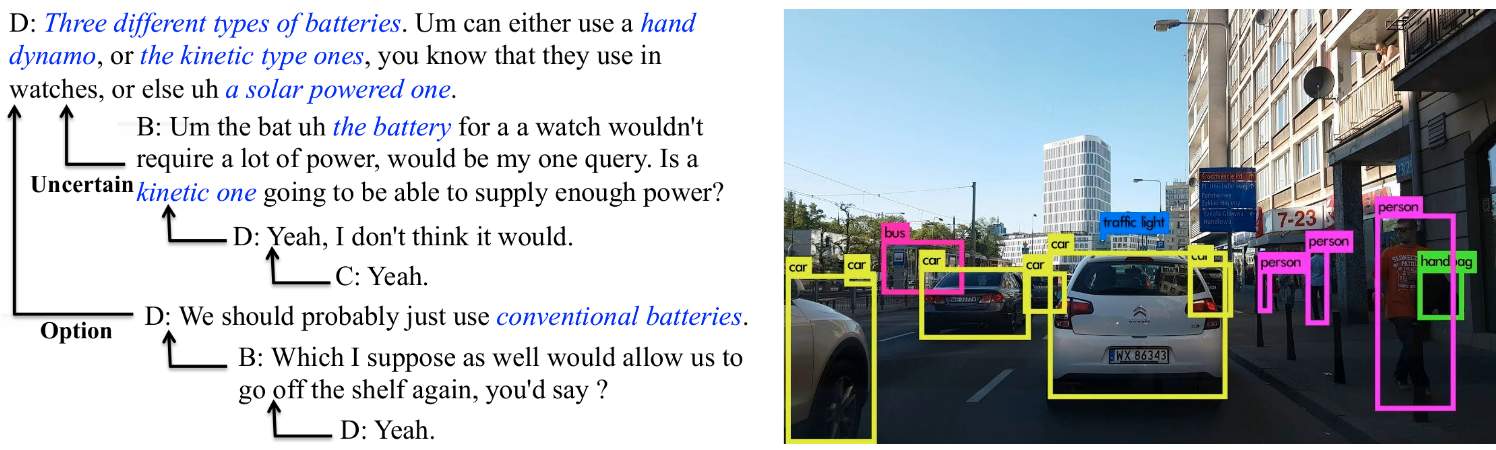
\includegraphics[width=1.0\columnwidth]{Images/intro_txt_car2.png} 
  \caption{\textbf{Left side:} A meeting snippet labeled with key discussion points (in blue) and discussion flow. Discussion flow, which is the latent information behind the text shows the structure of the discussion and the relation between two utterances. It helps with the identification of key discussion points. \textbf{Right side:} A sample image for object recognition task. We highlight bounding boxes and the label of each object. The bounding boxes are latent information and used to help identify objects.}
\end{figure}\label{fig:intro_car} 


Specifically, to capture a hidden state $z$, a mapping from input $x$ to learning target $y$ can be decomposed into two mappings: $z=f_1(x)$ and $y=f_2(z)$. Rather than modeling the distribution $p(y|x)$ directly, we can introduce an unobserved hidden variable $z$ to represent the intermediate state, and define two conditional distributions $p(z|x)$ and $p(y|z)$ for the data. The joint distribution over the target and hidden variable conditioned on the observed input can be written down as:

\[p(y,z|x) = p(y|z)p(z|x)\]

Usually, we can assume that $z$ is a discrete variable. By marginalizing out all possible state of $z$, we obtain the desired data distribution $p(y|x)$:

\[p(y|x) = \sum_z p(y|z)p(z|x)\] \label{eq2}

Model with hidden variables are known as latent variable models (LVM). Latent variable model is proposed to examine latent dependency structure among observable variables. The simplest form of LVM is when $z\in{1,...,K}$, representing a discrete latent state. We will use a discrete prior for this, $p(z_i)=Cat(\pi)$. For the likelihood, we use $p(x_i|z_i=k)=p_k(x_i)$, where $p_k$ is the k'th base distribution for the observations; this can be of any type \cite{murphy2012machine}. The overall model is known as a mixture model. The most widely used mixture model is the mixture Gaussians, also called a Gaussian mixture model (GMM). GMM is one of the most early works in introducing latent variables into machine learning models. Thereafter, latent variable modelling has gradually become an integral part of machine learning research. In text analysis, Probabilistic Latent Semantic Analysis (PLSA) \cite{hofmann2013probabilistic2} and Latent Dirichlet Allocation (LDA) \cite{blei2003latent} are two well-known topic modeling approaches, and both model the topic as a latent variable. In image analysis, it is natural to use latent variables to model human body parts or parts of objects in detection tasks. The work in \cite{wang2006hidden} introduces Hidden Conditional Random Fields, a discriminative probabilistic latent variable model for structured prediction, with applications to two computer vision tasks. 

In additional to these early LVM works, the combination of latent variable and neural networks has been widely studied in recent years. Chung \cite{chung2015recurrent} propose to integrate recurrent neural networks with latent random variables to model the kind of variability observed in highly structured sequential data. Ji \cite{ji2016latent2} presents a latent variable recurrent neural network architecture for jointly building a language model and understanding latent text information. Gulrajani \cite{gulrajani2016pixelvae2} introduced a VAE model for natural images to learn compressed representations in its latent variables by ignoring the small-scale structure in images. Inspired by all above work, in our thesis we study the usage of LVM with both traditional machine learning models and neural networks.

% LVM and deep learning...

% 2. learning :
% As latent variable models become more and more popular in machine learning community, different learning and inference methods are proposed to estimate model parameters...

For a better story structure, we divide the work into two parts based on two different types of latent information: \textit{sequential data} and \textit{discourse structure}. In chapter \ref{ch-2}, we will first introduce how to model sequential data as latent information in multi-label classification and knowledge based question answering. We analyze existing models proposed for these tasks, and show that existing training and prediction objectives are not well justified mathematically and have undesired consequences in practice. To avoid the drawbacks of existing ones, we develop efficient training and prediction methods by considering latent variables. We also crawl new datasets for multi-label prediction task, and release them for public research. Our experimental results show that our method outperforms state-of-the-art methods. 

In chapter \ref{ch-3}, we then study in natural language processing (NLP) how discourse structure contributes to understanding human language. Acquiring labeled discourse structures is a time-consuming process since it would require human annotators to inspect the full discourse. Therefore, we propose to model discourse structure as latent variable and jointly infer it with the learning target. In this way, we can solve the task without using additional annotations. Our models show good performances on two standard NLP tasks, text summarization and text based question answering. To further evaluate the correctness of generated discourse structures, we employ human identification and downstream tasks to interpret the output of our models. % Import your chapters here
\chapter{Sequential Data as Latent Variable} \label{ch-2}


Sequential Data is any kind of data where the order matters. Two types of sequential data are commonly studied in machine learning: \textit{sequence} and \textit{time-series}. A sequence is an ordered list of nominal values, while a time-series is an ordered list of numbers and is usually taken at successive equally spaced points in time. For instance, sequences are used to represent data such as sentences (sequences of words), while time-series are often used to represent data such as stock prices, temperature readings, and electricity consumption readings. 

When the training target is organized as a sequence, the model should not only learn the correct output combination, but also the ordering pattern. For example, in machine translation task, along with making a translation correct, the model should also find the best way to order each word in the translation. Different permutations of a sequence of words have very different meanings and readabilities in natural language. Similarly, in a motion planning system, a robot is trained to find a sequence of valid configurations that controls it to move from the source to the destination. Different orders of configurations (e.g. ``move up, move left'' and ``move left, move up'') generate different paths, and result in different interactions with the environment. In multi-label classification (studied in this chapter), different latent label orders lead different modeling outputs.

In our proposed system, the job of the base model is to generate $p(z|x)$, the probability of a latent sequence conditioned on the input. This step is usually called sequence prediction in machine learning, which uses historical sequence information to predict the next value or values in the future sequence. In addition to estimating $p(z|x)$ by using sequence prediction models, we also need to calculate the other term used in equation \ref{eq2}, i.e. $p(y|z)$. This calculation is usually modeled as a task to predict the target $y$ based on latent sequence $z$. We want $p(y|z)$ to be easily computable in this framework, and since $y$ is typically highly correlated with $z$ we will model it based on $z$. This is a key insight that motivates the latent variable paradigm. 


One of the most important topics in a machine learning task is the selection of the base model for comparison. Learning such models of sequences is a long-standing machine learning challenge and historically the domain of dynamic Bayesian networks (DBNs) such as hidden markov models (HMMs). The dominance of DBN-based approaches has been recently overturned by a resurgence of interest in neural network based approaches. A recurrent neural network (RNN) is able to encode the latent states into high-dimensional representations in a recurrent way, and then handle both variable-length input and output. The RNN model decomposes the joint probability over full latent sequence as a product of individual probability of each latent value in the sequence based on chain rule. Most recently, Neural Transformer \cite{vaswani2017attention}, improved from RNN, removes the dependency between adjacent RNN nodes, and allows each node to directly condition on every previous node (not just the previous one). In figure \ref{fig:model_c2}, we show the model architectures of HMM and RNN. As we can see, they both consist of two parts: (1) a transition function that determines the evolution of the internal state representation (i.e. $s_i=f(s_{i-1})$ and $h_i=f(h_{i-1})$), and (2) a mapping from the state to the output (i.e. $x_i=f(s_i)$ and $y_i=f(h_i)$). Advantages of using NN models over DBNs is that DBNs have typically been limited either to relatively simple state transition structures or to relatively simple internal state structure (e.g., the HMM state space consists of a single set of mutually exclusive states). In other words, NN based models are more powerful and capable of learning a better representations compared to DBNs. We use RNN and Transformer as our base models.

\begin{figure}[t] 
\centering
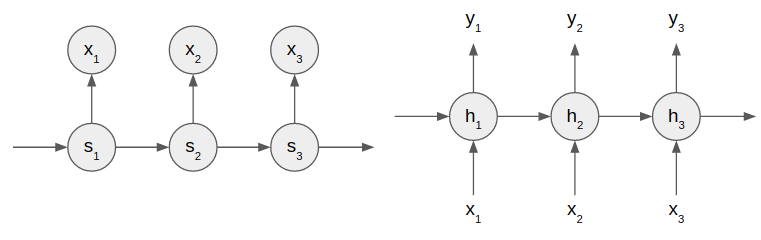
\includegraphics[width=1.0\columnwidth]{Images/rnn_hmm.png} 
  \caption{We plot the structure of HMM in the left side and RNN in the right side. For simplicity, we omit some parameters in the model. HMM is a generative model, where $x$ represents the observation and $s$ represents the hidden state. RNN is a discriminative model, where $x$ represents input features, $h$ represents hidden state representation, and $y$ represents model outputs.}
\end{figure}\label{fig:model_c2} 

Many recent work studying latent sequential data with RNN focuses on adding uncertainty to the hidden states $h$ of the models. Inspired by variational autoencoder, Chung \cite{chung2015recurrent} first propose to use high-level latent random variables to model the kind of variability observed in highly structured sequential data. Following this idea, Fraccaro \cite{fraccaro2016sequential} explicitly add a stochastic layer to RNN to model uncertainty of RNN hidden states. In their setup, latent variable $z$ is just a sequence of hidden representations of input $x$, e.g. $z$ is a vector representation of input waveform in speech recognition task. On the contrary, the other line of studying latent sequential data is to explicitly translate latent sequence $z$ into interpretable variables or features. Our work falls into the later track. To solve real-world tasks, we manage to find the interpretable intermediate state to bridge the gap between input and output, and also integrate the domain knowledge and task-specific constraints together to build an end-to-end solution. Specifically, we investigate the interpretation of z and its possible values that connect input $x$ and output $y$, and propose novel approaches to make our model fit to real world tasks, such as handling inputs from multiple sources or regularizing contributions of different features.


In this chapter, we focus on discussing latent sequence in two text-based real world tasks, where sequential latent information are utilized. In section \ref{sec:2-1}, we first study a scenario that a set prediction problem being decomposed into latent sequence prediction problem in multi-label classification, and then in section \ref{sec:2-2} we discuss how a similar idea can be used to solve knowledge based question answering task (KBQA).


\section{Latent Label Order in Multi-label Classification} \label{sec:2-1}

\subsection{Background}

Multi-label text classification is an important machine learning task wherein one must predict a set of labels to associate with a given document; for example, a news article might be tagged with labels \texttt{sport}, \texttt{football}, \texttt{2018 world cup}, and \texttt{Russia}. Formally, we are given a set of label candidates $\mathcal{L}=\{1,2,...,L\}$, and we aim to build a classifier which maps a document $x$ to a set of labels $\mathbf{y}\subset \mathcal{L}$. The label set $\mathbf{y}$ is typically written as a binary vector $\mathbf{y}\in \{0,1\}^L$, with each bit $y_{\ell}$ indicating the presence or absence of a label.

In multi-label prediction, labels often exhibit complex dependencies: knowing some labels---such as \texttt{sport} and \texttt{football}---should make it easier to predict \texttt{2018 world cup} and then \texttt{Russia}. There are several methods that manage to capture label dependencies by building a joint probability estimation over all labels $p(\mathbf{y}=(y_1,y_2,...,y_L)|x)$ \cite{ghamrawi2005collective,read2009classifier,DBLP:conf/icml/DembczynskiCH10,li2016conditional}. 
% \kechen{put BR before the introduction of dependency? because there is nothing about dependency by using BR} 
The most popular approach is to model multi-label prediction as a sequence prediction task. This is usually obtained by assigning the labels a globally fixed order (e.g.\ by label frequency), and learning labels one-by-one. In this way, the prediction of a single label is dependent on the prediction in the earlier sequence. Recently, RNNs become one of the most popular sequence prediction models, and have been applied to multi-label classification \cite{DBLP:conf/cvpr/WangYMHHX16,DBLP:journals/corr/ZhangWSZL16,DBLP:conf/icpr/JinN16,DBLP:conf/iccv/WangCLXL17,DBLP:journals/corr/abs-1709-08553,DBLP:conf/aaai/ChenCYW18,DBLP:journals/corr/abs-1806-04822}.  

To review how RNN can be used to solve a sequence prediction task, let $\mathbf{s}=(s_1,s_2,...,s_T)$ be an input sequence of outcomes, in a particular order, where $s_t \in \{1,2,...,L\}$; the order is often critical to the datapoint. An RNN model defines a probability distribution over all possible output sequences given the input in the form $p(\mathbf{s}=(s_1,s_2,...,s_T)|x)=\prod_{t=1}^T p(s_t|x,s_1,s_2,...,s_{t-1})$. To train the RNN model, one maximizes the likelihood of the ground truth sequence. %$p(\mathbf{s}=(s_1,s_2,...,s_T)|x)$.
At prediction time, one seeks to find the sequence with the highest probability $\mathbf{s}^*=\arg\max_\mathbf{s} p(\mathbf{s}|x)$, and this is usually implemented approximately with a beam search procedure \cite{lowerre1976harpy}. The sequence history is encoded with an internal memory vector $h_t$ which is updated over time. RNN is also often equipped with the attention mechanism \cite{DBLP:journals/corr/BahdanauCB14}, which in each timestep $t$ puts different weights on different words (features) and thus effectively attends on a list of important words. The context vector $c_t$ is computed as the weighted average over the dense representation of important words to capture information from the document. The context $c_t$, the RNN memory $h_t$ at timestep $t$, and the encoding of previous label ${s_{t-1}}$ are all concatenated and used to model the label probability distribution at time $t$ as $p(s_t|x,s_1,s_2,...,s_{t-1}) \sim \softmax(\phi(c_t,h_t,s_{t-1}))$, where $\phi$ is a non-linear function, and $\softmax$ is the normalized exponential function. RNN is trained with the standard maximum likelihood objective \cite{DBLP:conf/nips/NamMKF17}: 
\begin{align}
\maximize \sum_{n=1}^N \log p(\mathbf{s}^{(n)}|x^{(n)})
\label{eq:standard_rnn}
\end{align}
where $x^{(n)}$ is the $n$-th document and $N$ is the total number of documents in the corpus. 

One of the challenges of mapping a set to a sequence is to determine the appropriate label order. Vinyals \cite{vinyals2015order} proposes to dynamically choose during training the sequence order deemed as most probable by the current RNN model:
\begin{align}
\maximize \sum_{n=1}^N \max_{\mathbf{s}\in \pi(\mathbf{y}^{(n)})}\log p(\mathbf{s}|x^{(n)})
\label{eq:max_obj}
%\vspace{-2ex}
\end{align}
where the $\pi(\mathbf{y}^{(n)})$ stands for all permutations of the label set $\mathbf{y}^{(n)}$. This eliminates the need to manually specify the label order.
However, as noticed by the authors, this objective cannot be used in the early training stages: the early order choice (often random) is reinforced by this objective and can be stuck upon permanently. To address this issue, Vinyals \cite{vinyals2015order}~also proposes two smoother alternative objectives to initialize the model training:

The authors suggest that one first consider many random orders for each label set in order to explore the space:
\begin{align}
\maximize \sum_{n=1}^N \sum_{\mathbf{s}\in \pi(\mathbf{y}^{(n)})}\log p(\mathbf{s}|x^{(n)})
\label{eq:wrong_obj}
\end{align} 

After that, one can sample sequences following the model predictive distribution instead of uniform distribution:
\begin{align}
\maximize \sum_{n=1}^N \sum_{\mathbf{s}\in \pi(\mathbf{y}^{(n)})}p(\mathbf{s}|x^{(n)})\log p(\mathbf{s}|x^{(n)})
\label{eq:sample_obj}
\end{align} 

In training, one needs to schedule the transition among these objectives, a rather tricky endeavor. At prediction time, one needs to find the most probable set. This is done by (approximately) finding the most probable sequence $\mathbf{s}^*=\arg\max_\mathbf{s} p(\mathbf{s}|x)$ and treating it as a set $\hat{\mathbf{y}}=set(\mathbf{s}^*)$. With a large number of sequences, it is quite possible that the argmax has actually a low probability, which can lead to neglecting important information when we ignore sequences other than the top one.



\subsection{Decomposing Multi-label Set Prediction into Sequence Permutations Prediction}

We propose a new way of adapting RNN to multi-label set prediction, which we call \emph{set-RNN}. We appreciate the RNN model structure \cite{rumelhart1988learning} (defines a probability distribution over all possible sequences directly) and introduce training and prediction objectives tailored for sets that take advantage of it, while making a clear distinction between the sequence probability $p(\mathbf{s}|x)$ and the set probability $p(\mathbf{y}|x)$. 
 We define the set probability as the sum of sequences probabilities for all sequence permutations of the set, namely $p(\mathbf{y}|x)=\sum_{\mathbf{s}\in \pi(\mathbf{y})} p(\mathbf{s}|x)$. Based on this formulation, an RNN also defines a probability distribution over all possible sets indirectly since $\sum_{\mathbf{y}} p(\mathbf{y}|x)=\sum_{\mathbf{y}}\sum_{\mathbf{s}\in \pi(\mathbf{y})} p(\mathbf{s}|x)=\sum_{\mathbf{s}} p(\mathbf{s}|x)=1$. This formula can also be interpreted as a latent variable objective: $p(\mathbf{y}|x)=\sum_{\mathbf{s}\in \pi(\mathbf{y})} p(y|\mathbf{s})p(\mathbf{s}|x)$, where the label order $\mathbf{s}$ is seen as a latent variable and $\pi(\mathbf{y})$ is a set including all possible latent states. Because the process of mapping a sequence to a set does not contain any uncertainty, the probability $p(y|\mathbf{s})$ equals to 1. Then we can ignore this term from the latent variable objective. In standard maximum likelihood training, one wishes to maximize the likelihood of given label sets, namely, $\prod_{n=1}^N p(\mathbf{y}^{(n)}|x^{(n)})=\prod_{n=1}^N \sum_{\mathbf{s}\in \pi(\mathbf{y}^{(n)})} p(\mathbf{s}|x^{(n)})$, or equivalently, 
\begin{align}
\maximize \sum_{n=1}^N \log \sum_{\mathbf{s}\in \pi(\mathbf{y}^{(n)})} p(\mathbf{s}|x^{(n)})
\label{eq:right_obj}
\end{align}


%This training objective (\ref{eq:right_obj}) looks similar to the objective (\ref{eq:wrong_obj}) considered in previous work \cite{vinyals2015order}, but in fact they correspond to very different transformations. Under the maximum likelihood framework, our objective (\ref{eq:right_obj}) corresponds to the transformation $p(\mathbf{y}|x)=\sum_{\mathbf{s}\in \pi(\mathbf{y})} p(\mathbf{s}|x)$, while objective (\ref{eq:wrong_obj}) corresponds to the transformation $p(\mathbf{y}|x)=\prod_{\mathbf{s}\in \pi(\mathbf{y})} p(\mathbf{s}|x)$. The latter transformation does not define a valid probability distribution over $\mathbf{y}$ (i.e., $\sum_{\mathbf{y}} p(\mathbf{y}|x)\neq 1$), and it has an undesired consequence in practical model training: because of the multiplication operation, the RNN model has to assign equally high probabilities to all sequence permutations of the given label set in order to maximize the set probability. If only some sequence permutations receive high probabilities while others receive low probabilities, the set probability computed as the product of sequence probabilities will still be low. In other words, if for each document, RNN finds one good way of ordering relevant labels (such as hierarchically) and allocates most of the probability mass to the sequence in that order, the model still assigns low probabilities to the ground truth label sets and will be penalized heavily. As a consequence the model has little freedom in discovering and concentrating on some natural label order. In contrast, with our proposed training objective, in which the multiplication operation is replaced by the summation operation, it suffices to find only one reasonable permutation of the labels for each document. It is worth noting that different documents can have different label orders; thus our proposed training objective gives the RNN model far more freedom on label order. The other two objectives (\ref{eq:max_obj}) and (\ref{eq:sample_obj}) proposed in \cite{vinyals2015order} are less restrictive than (\ref{eq:wrong_obj}), but they have to work in conjunction with (\ref{eq:wrong_obj}) because of the self reinforcement issue. Our proposed training objective has a natural probabilistic interpretation, and does not suffer from self reinforcement issue. Thus it can serve as a stand alone training objective. Also, using Jensen’s inequality, one can show that objective (\ref{eq:wrong_obj}) is maximizing a lower bound on the log-likelihood, while objective (\ref{eq:right_obj}) is maximizing it directly. 

\begin{algorithm}[ht]
  \SetKwInOut{Input}{Input}
  \SetKwInOut{Output}{Output}

  % \underline{function Beam\_Search\_for\_Given\_Set} $(\mathbf{y},m)$\;
  \Input{Instance $x$ \\
  Subset of labels considered $G\subset \mathcal{L}$\\
  Boolean flag $ALL$: 1 if sequences must contain all $G$ labels; 0 if partial sequences are allowed }
  \Output{A list of top sequences and the associated probabilities} 
  Let $\mathbf{s}_1$,$\mathbf{s}_2$,...,$\mathbf{s}_K$ be the top $K$ sequences found so far. Initially, all $K$ sequences are empty. $\oplus$ means concatenation. \\
  % Let $C$ be the set of candidate sequences, initially empty.\\
  \While {true}{
   // Step 1: Generate Candidate Sequences from each existing sequence $s_k \in K$ and all possible new labels $l \in G$:\\
  Expand all non-stopped sequences:\\
   % $C = \{ \mathbf{s}_k\oplus l | l\in G, l \notin s_k, STOP \notin s_k \}$\\
   $C = \{ \mathbf{s}_k\oplus l | l\in G, STOP \notin s_k \}$\\  
Include stopped sequences:\\
  $C = C \cup \{ \mathbf{s}_k | STOP \in s_k \}$\\
  Terminate non-stopped sequences:\\
  \If{$ALL==0$}{
  % Add $\mathbf{s}_k\oplus STOP$ to $C$ }
  %
  $C =C \cup \{ \mathbf{s}_k\oplus STOP | STOP \notin s_k \}$
  }


 // Step 2: Select highest probabilities sequences from candidate set $C$\\
  % From the candidate set $C$ generated by all $\mathbf{s}_k$ in Step 1, select the top $K$ candidates with the highest probabilities and use them as new values for $\mathbf{s}_1$,$\mathbf{s}_2$,...,$\mathbf{s}_K$\\
  $K$
  % = \{$\mathbf{s}_1$,$\mathbf{s}_2$,...,$\mathbf{s}_K$\}
  = topK-argmax$_k \{\text{prob}[s_k] | s_k \in C\}$\\
  \If {all top $K$ sequences end with $STOP$ or contain all labels in $G$}{
  Terminate the algorithm}

    % \tcp{Prune sequence list to }
    % $s \leftarrow s_{ij}[:k_3]$
   }
  \Return{sequence list $\mathbf{s}_1$,$\mathbf{s}_2$,...,$\mathbf{s}_K$ and the associated probabilities}
  \caption{Beam\_Search}
  \label{alg:beam_combine}
\end{algorithm}

Training an RNN model with the proposed objective (\ref{eq:right_obj}) requires summing up sequence (permutation) probabilities for a set $\mathbf{y}$, where $|\mathbf{y}|$ is the cardinality of the set. Thus evaluating this objective exactly can be intractable. We can approximate this sum by only considering the top $K$ highest probability sequences produced by the RNN model. We introduce a variant of beam search for sets with width $K$ and with the search candidates in each step restricted to only labels in the set (see Algorithm~\ref{alg:beam_combine} with $ALL=1$)%\footnote{The ``ALL'' flag determines if the sequences can terminate with a partial subset of labels (as used in Algorithm~\ref{alg:test} line 2) or a full set is required (as used in Algorithm~\ref{alg:train_beam} line 4 and Algorithm~\ref{alg:test} line 7).}
. This approximate inference procedure is carried out repeatedly before each batch training step, in order to find highest probability sequences for all training instances occurring in that batch. The overall training procedure is summarized in Algorithm \ref{alg:train_beam}.

The transformation $p(\mathbf{y}|x)=\sum_{\mathbf{s}\in \pi(\mathbf{y})} p(\mathbf{s}|x)$ also naturally leads to a prediction procedure, which is different from the previous standard of directly using most probable sequence as a set. We instead aim to find the most likely set $\hat{\mathbf{y}}=\arg\max_{\mathbf{y}} p(\mathbf{y}|x)$. %The most probable set may not correspond to the most probable sequence; these are certainly cases where our method has an advantage. 
Both our method and the competitor state-of-the-art (Vinyals-RNNs) are at most $K$ times slower than a vanilla-RNN,  due to the time spent on dealing with $K$ permutations per datapoint. 

\begin{algorithm}
  \SetKwInOut{Input}{Input}
  \SetKwInOut{Output}{Output}

 % \underline{function Euclid} $(a,b)$\;
  \Input{Multi-label dataset $(x^{(n)},\mathbf{y}^{(n)}),n=1,2,...,N$ }
  \Output{Trained RNN model parameters}
  
  % Initialize model parameters\\
  \ForEach {batch}{
    % \ForEach {batch }{
      \ForEach{$(x^{n},\mathbf{y}^{n})$ in the batch}{
        Get top $K$ sequences :\\
		  	$\{\mathbf{s}^n_{1},...,\mathbf{s}^n_{K}, p(\mathbf{s}^n_{1}|x^n),...,p(\mathbf{s}^n_{K}|x^n)\}$= Beam\_Search$(x^{n},\mathbf{y}^{n}, ALL=1$)\\
        }
      Update model parameters by maximizing $\sum\limits_{(x^{n},\mathbf{y}^{n}) \in \text{batch}} \log \sum\limits_{\mathbf{s}\in\{\mathbf{s}^n_{1},...,\mathbf{s}^n_{K}\}} p(\mathbf{s}|x^{n})$
    % }
  }
  \caption{Training method for set-RNN}
  \label{alg:train_beam}
\end{algorithm}

We test our proposed set-RNN method on 4 real-world multi-label classification datasets, RCV1-v2, Slashdot, TheGuardian, and Arxiv Academic Paper Dataset (AAPD) \cite{DBLP:journals/corr/abs-1806-04822}. We adopt \emph{label-F1} (average F1 over labels) and \emph{instance-F1} (average F1 over instances) as our main evaluation metrics, as defined below:
 
\begin{align*} \text{label-F1} = \frac{1}{L}\sum_{\ell=1}^L\frac{2\sum_{n=1}^N y^{(n)}_\ell \hat{y}^{(n)}_\ell}{\sum_{n=1}^N y^{(n)}_\ell+\sum_{n=1}^N \hat{y}^{(n)}_\ell}\\
\text{instance-F1} = \frac{1}{N}\sum_{n=1}^N\frac{2\sum_{\ell=1}^L y^{(n)}_\ell \hat{y}^{(n)}_\ell}{\sum_{\ell=1}^L y^{(n)}_\ell+\sum_{\ell=1}^L \hat{y}^{(n)}_\ell}
\end{align*}
where for each instance $n$, $y_\ell^{(n)}=1$ if label $\ell$ is a given label in ground truth; $\hat{y}_\ell^{(n)}=1$ if label $\ell$ is a predicted label.


\begin{table*}[ht]
	\begin{center}
	\resizebox{1.0\columnwidth}{!}{%resize the table
		\begin{tabular}{|l|cc|cc|cc|cccc|}
			\hline
			\multirow{2}{*}{Methods}	& 
       \multicolumn{2}{c|}{Slashdot}&\multicolumn{2}{c|}{RCV1-v2}&\multicolumn{2}{c|}{TheGuardian}&\multicolumn{4}{c|}{AAPD} \\
       \cline{2-11}
      & label-F1 & instance-F1 & label-F1 & instance-F1 & label-F1 & instance-F1 & label-F1 & instance-F1 & hamming-loss & micro-F1 \\

            \hline
      BR
      & .271 & .484 & .486 & .802 &.292 & .572 & .529 & .654 & .0230 & .685 \\
    %  BR-support
     % & .247 & .516 & .486 & .805 &.296 & .594 & .545 & .689 & \textbf{.0228} & .696\\
      PCC 
      & .279 & .480 & .595 & .818 &- & - & .541 & .688 & .0255 & .682 \\
      seq2seq-RNN 
       & .270 & .528 & .561 & .824 &.331 & .603 & .510 & .708 & .0254 & .701 \\
    %  Vinyals-RNN-uniform 
    %   & .279 & .527 & .578 & .826 & .313 & .567 & .532 & .721 & .0241 & .711\\
    %  Vinyals-RNN-sample
    %  & .300 & .531 & .590 & .828 & .339 & .597 & .527 & .706 & .0259 & .697 \\
      Vinyals-RNN-max
      & .293 & .530 & .588 & .829 & .343 & .599 & .535 & .709 & .0256 & .700 \\
  %    Vinyals-RNN-max-direct
  %     & .226 & .518 & .539 & .808 & .313 & .583 & .490 & .702 & .0257 & .694\\
      SGM
      &-&-&-&-&-&-& - & - & .0245 & .710 \\
      set-RNN 
       & \textbf{.310} & \textbf{.538} & \textbf{.607} & \textbf{.838} &\textbf{.361} & \textbf{.607} & \textbf{.548} & \textbf{.731} & .0241 & \textbf{.720}\\
      \hline

		\end{tabular}
		}
	\end{center}
	\caption{Comparison of different approaches. ``-'' means result not available. For \emph{hamming loss}, the lower the value is, the better the model performs. For all other measures, the higher the better.%\kechen{cardinality analysis, V's method can't perform well on Guardian. why?}
  }\label{tab:main}
\end{table*}

Table \ref{tab:main} shows the performance of different methods in terms of \emph{label-F1} and \emph{instance-F1}. We select two traditional multi-label classifiers and three RNN-based multi-label solutions as baselines in the experiment. Introduction of these methods can be found in appendix \ref{multi-baseline}. The SGM results are taken directly from \cite{DBLP:journals/corr/abs-1806-04822}, and are originally reported only on AAPD dataset in terms of \emph{hamming-loss} and \emph{micro-F1}. Definitions of these two metrics can be found in \cite{koyejo2015consistent}. Our method performs the best in all metrics on all datasets (except hamming loss on AAPD, see table \ref{tab:main}). In general, RNN based methods perform better than traditional methods BR, BR-support and PCC. Among the Vinyals-RNN variants, Vinyals-RNN-max and Vinyals-sample work the best and have similar performance. However, they have to be initialized by Vinyals-RNN-uniform. Otherwise, the training gets stuck in early stage and the performance degrades significantly. One can see the clear degradation by comparing the Vinyals-RNN-max row (with initialization) with the Vinyals-RNN-max-direct row (without initialization). By contrast, our training objective in set-RNN does not suffer from this issue and can serve as a stable stand alone training objective. On TheGuardian dataset, set-RNN performs slightly better than seq2seq-RNN in terms of instance-F1, but much better in terms of label-F1. It is known that instance-F1 is basically determined by the popular labels' performance while label-F1 is also sensitive to the performance on rare labels. Figure~\ref{fig:labelf1} shows that set-RNN predicts rare labels better than seq2seq-RNN.

\begin{figure}[t]
\centering
%\hspace{-2ex}
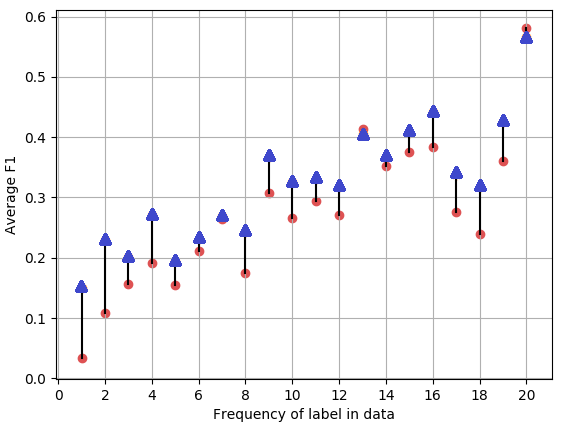
\includegraphics[width=0.5\columnwidth]{Images/labelf1_v2.png}
\caption{Average F1 over rare labels with the same frequency on TheGuardian dataset. Blue($\Delta$)=set-RNN, Red($\cdot$)=seq2seq-RNN.}
\label{fig:labelf1}
%\vspace{-6ex}
\end{figure}


\begin{figure}[t]
\centering
%\hspace{-2ex}
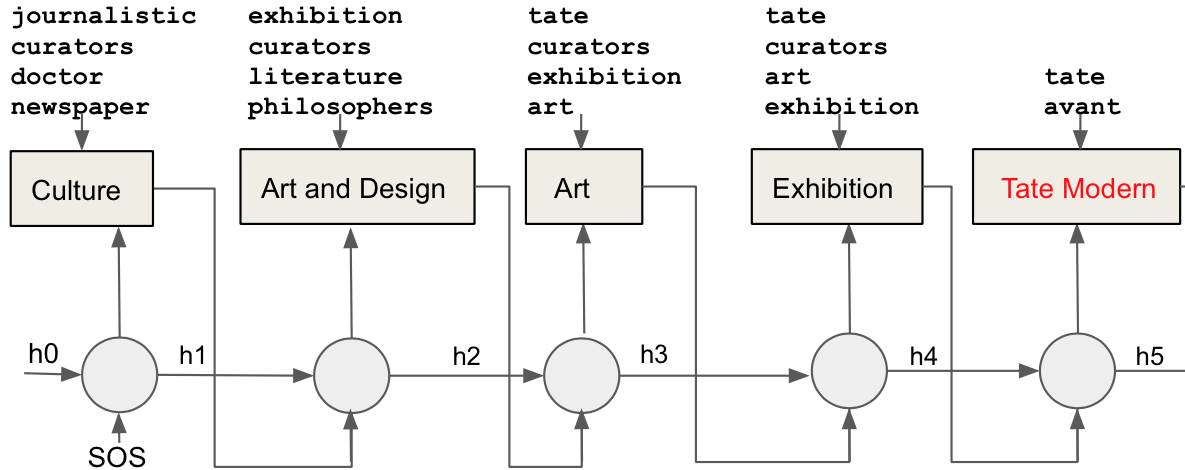
\includegraphics[width=0.8\columnwidth]{Images/train_sequence.png}
%\vspace{-4ex}
%\hspace{-2ex}
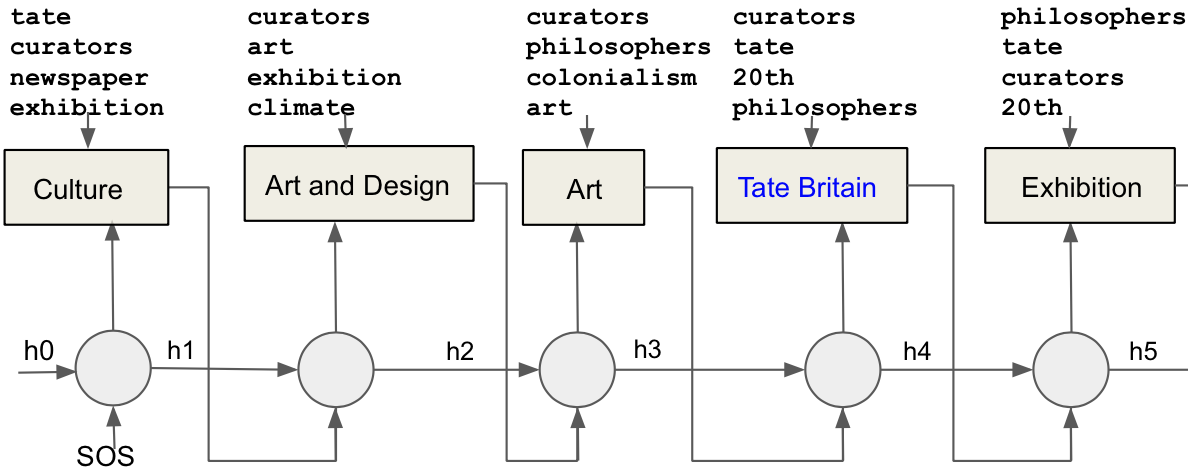
\includegraphics[width=0.8\columnwidth]{Images/train_set.png}

\caption{Top: best sequence by seq2seq-RNN; bottom: best sequence by set-RNN. Above models, at each time, we list the top unigrams selected by attention.}
\label{fig:models}
%\vspace{-6ex}
\end{figure}
We further demonstrate how latent label order helps in multi-label classification task with an example from TheGuardian\footnote{\scriptsize This document can be viewed at \url{http://www.guardian.co.uk/artanddesign/jonathanjonesblog/2009/apr/08/altermodernism-nicolas-bourriaud}}. Modeling label order as a latent variable relaxes the constraint that a model has to be trained in a given fixed label order. Figure~\ref{fig:models} shows the predictions made by standard RNN that simply mapping a label set to a sequence based on label frequencies (we will call this method seq2seq-RNN) and our method. In this particular example, the top sequence agrees with the top set in our method's prediction so we can just analyze the top sequence. seq2seq-RNN predicts \texttt{Tate Modern} (incorrect but more popular label) while we predict \texttt{Tate Britain} (correct but less popular label). The seq2seq predicted sequence is in the decreasing label frequency order while our predicted sequence is not. In the training data, \texttt{Exhibition} is more frequent than \texttt{Tate Britain} and \texttt{Tate Modern}. If we arrange labels by decreasing frequency, \texttt{Exhibition} is immediately followed by \texttt{Tate Modern} 19 times, and by \texttt{Tate Britain} only 3 times. So it is far more likely to have \texttt{Tate Modern} than \texttt{Tate Britain} after \texttt{Exhibition}. However, at the set level, \texttt{Exhibition} and \texttt{Tate Modern} co-occurs 22 times while \texttt{Exhibition} and \texttt{Tate Britain} co-occurs 12 times, so the difference is not so dramatic. In this case, imposing the sequence order biases the probability estimation and leads to incorrect predictions.
%We further demonstrate how set-RNN works with two examples. In the first example from the RCV1-v2 dataset, the most probable set predicted by set-RNN (which is also the correct set in this example) does not come from the most probable sequence. Top sequences in decreasing probability order are listed in Table~\ref{tab:pred_case_study}. The correct label set \{forex, markets, equity, money markets, metals trading, commodity\} has the maximum total probability of 0.161, but does not match the top sequence.

\section{Latent Reasoning Path in Knowledge based Question Answering}\label{sec:2-2}

\subsection{Background}

Knowledge-based question answering (KBQA) is the task of finding answers to questions by processing a structured knowledge base $\mathcal{KB}$. %where the beliefs are stored as triples containing two entities and the relation linking them. 
A $\mathcal{KB}$ consists of a set of entities $\mathcal{E}$, a set of relations $\mathcal{R}$, and a set of literals $\mathcal{S}$. A knowledge base fact is defined as $(h,r,t)$, where $h\in \mathcal{E}$ is the head entity, $t \in \mathcal{E} \bigcup \mathcal{S}$ is the tail entity/literal, and $r\in \mathcal{R}$ is the directed relation between $h$ and $t$. To answer a simple single-relation question (\emph{i.e.} a 1-hop question) such as: \textit{``Who is the president of the United States?''}, a typical KBQA system first identifies the entity (\emph{i.e.} ``United States'') and the relation (\emph{i.e.} ``president'') asked in the question, and then searches for the answer entity by matching the entity-relation tuple <United States, president, ?> over $\mathcal{KB}$.

While a single-hop question can be answered by searching a predicate relation in $\mathcal{KB}$, it is much harder to answer more complex multi-hop questions containing multiple entities and relations with constraints. For complex questions, it is not easy to extract all the relations correctly together with their head and tail entities in the right order. Most prior work on multi-hop KBQA focus on learning a single given ground truth reasoning path for each question, and outputting the most possible reasoning path during prediction \cite{DBLP:conf/coling/ZhouHZ18,DBLP:journals/corr/abs-1801-09893,DBLP:conf/adbis/YuHYZW18,DBLP:conf/ijcai/LanW019}. However, it is common that $\mathcal{KB}$ has many alternative paths leading to the correct answer, of various reasoning qualities. These alternative reasoning paths are usually not provided as ground truth by the human annotators. Or there is no any labeled path in the given dataset at all, because in practice questions and answers are easy to collect (sometimes for free), but path annotation is very labor-intensive and expensive. 

\begin{figure}[t]
 \centering
 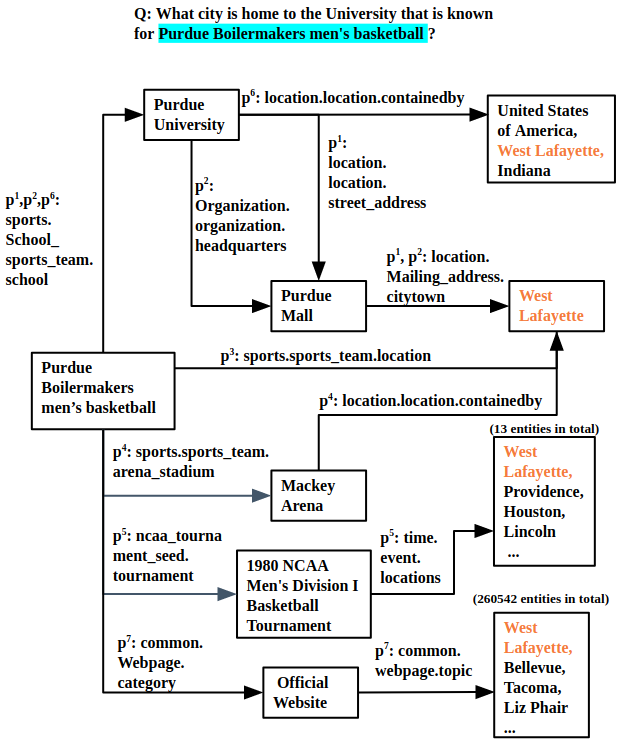
\includegraphics[width=0.7\linewidth]{Images/fig1.png}
 \caption{One QA example with Multiple Reasoning Paths from \textsc{ComplexWebQuestion}-1.1. The blue color highlighted is the extracted topic entity. Each square represents an entity, and the arrows represent the relations. Reasoning path $\mathbf{p}^1$ to $\mathbf{p}^4$ are the correct ones containing meaningful reasoning paths to the final answer. $\mathbf{p}^5$ and $\mathbf{p}^6$ are the ``second choice'' paths that generate a larger final answer set containing some wrong entities. $\mathbf{p}^7$ is the wrong one as its reasoning path is totally not interpretable and the answer set is huge.}
 \label{QAPaths}
\end{figure}

For example, Figure \ref{QAPaths} shows 7 reasoning paths $\mathbf{p}^n={e^n_0\rightarrow r^n_1 \rightarrow e^n_1 \rightarrow \cdots \rightarrow e^n_{ans}}\ (n=\lbrace 1, \dots, 7 \rbrace)$ leading to an answer set containing the correct answer \textit{``West Lafayette''} for a given question \textit{``What city is home to the University that is known for Purdue Boilermakers men's basketball?''}, but only the reasoning path $\mathbf{p}^1$ is labeled as the correct path in the dataset \cite{DBLP:journals/corr/abs-1807-09623}. Actually, there are four paths ($\mathbf{p}^1$,$\mathbf{p}^2$,$\mathbf{p}^3$,$\mathbf{p}^4$) pointing to the exact answer set containing only the answer entity, and thus can be treated as ground truth paths when training. A model trained with only $\mathbf{p}^1$ as supervision is likely to miss other paths which are also valid. For example, it will probably map a similar question \textit{``What city is home to the stadium that is known for Los Angeles Lakers?''} to path $\mathbf{p}^1$, but fail to associate it with $\mathbf{p}^3$ or $\mathbf{p}^4$, because $\mathbf{p}^3$ or $\mathbf{p}^4$ contain different types of relations. However, $\mathbf{p}^1$ is a wrong reasoning path for that test question.

We propose to model the reasoning path as a latent variable and the answer as the training target. In our system, we do not require any labeled paths in the training set, which significantly reduce the work of annotators. We want to see that our model can output correct answer, as well as reasonable paths leading to the answer. This framework can be learned with any base model. Following the previous multi-label task, we select RNN as our base model.

\subsection{Reasoning path Prediction Model}

\begin{figure*}[t]\centering
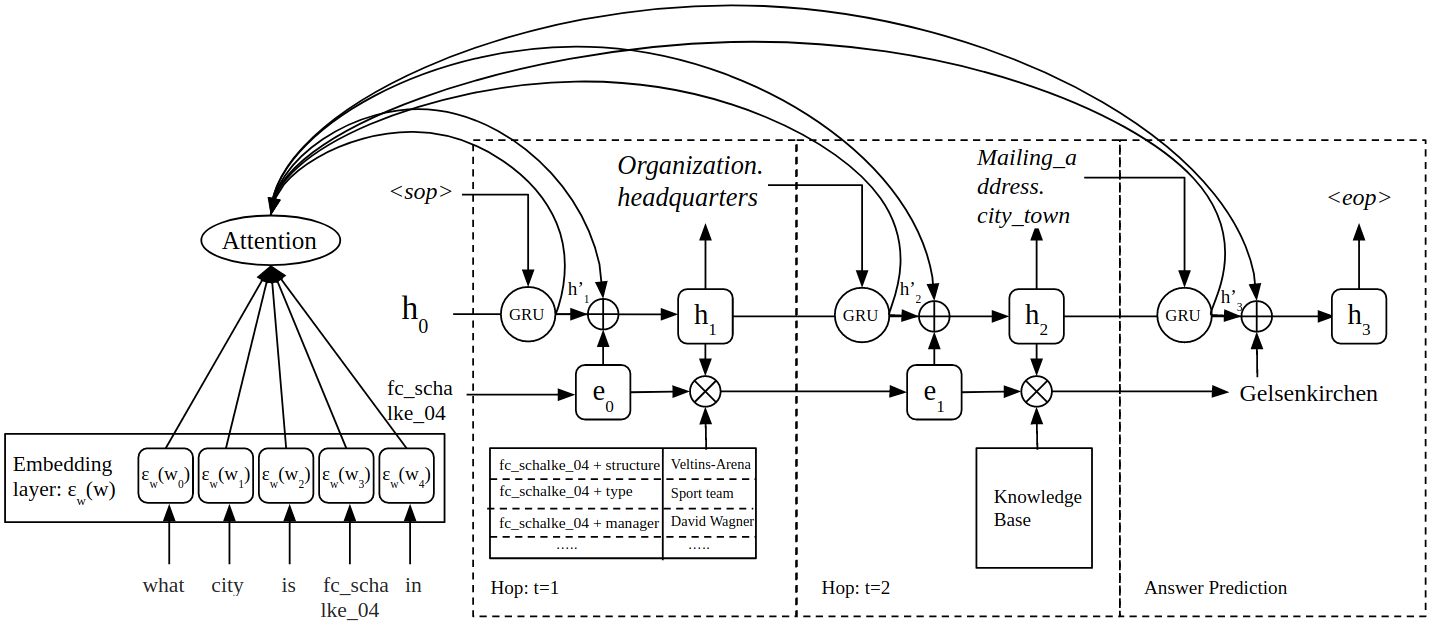
\includegraphics[width=1.0\columnwidth]{Images/model.png}
\caption{An illustration of how our model works with a QA pair \textit{``What city is fc\_schalke\_04 in?''} and \textit{Gelesenkirchen}. The entity linker extracts \textit{fc\_schalke\_04} as the topic entity. We only show one possible paths here: $r_1$ is \textit{Organization.headquarters} and $r_2$ is \textit{Mailing\_address.city\_town}, our model can be used to output the probability of this given path. The symbol $\bigoplus$ represents concatenation, and $\bigotimes$ represents knowledge base lookup. }
\label{fig:model}
\end{figure*}


We first introduce some notations. For a given question $q$ and its topic entity $e_0$ (identified by entity linking tool), a reasoning path is a sequence in the form $\mathbf{p} = (e_0, r_{1},e_{1},r_{2}, \cdots,e_{T-1}, r_{T})$ that points to the answer entity $e_T=y$. That is, $\mathbf{p}\rightarrow e_T=y$. Each step $(e_{t-1},r_t,e_t)$ is a valid fact in the knowledge base $\mathcal{KB}$. We assume that there are multiple valid paths $\mathbf{p}\in \mathcal{P}$ that can lead to the correct answer $y$ and they are not given by the annotator in the dataset. We treat these paths as hidden variables and we marginalize them out to compute the probability of getting the answer $y$:

\begin{align}
&p(y|q)\nonumber=\sum_{\mathbf{p}\in\mathcal{P}} [p(e_{T(\mathbf{p})}=y|\mathbf{p},q)p(\mathbf{p}|q)] \nonumber
=\sum_{\mathbf{p}\in\mathcal{P}}\prod_{t=1}^{T(\mathbf{p})} [p(e_t|e_{t-1},r_t) p(r_t|q,e_0,r_1,\cdots,e_{t-1})]
\label{eq:marginal}
\end{align}
where $\mathcal{P}$ is a set of all valid paths leading to the answer $y$, and $T(\mathbf{p})$ is the number of hops in the path $\mathbf{p}$.

Given this training objective, we want to calculate the value of two terms, $p(e_{T(\mathbf{p})}=y|\mathbf{p},q)$ and $p(\mathbf{p}|q)$. Solving the probability of latent variable $\mathbf{p}$ conditioned on $q$ can be seen as a sequence prediction task. Figure \ref{fig:model} illustrates the architecture of our model. We integrate the $\mathcal{KB}$ and the entity representations into the RNN model. At a timestep $t$, the input hidden representations of GRU unit and predicted relation are denoted by $h_{t-1}$ and $r_t$ respectively. The model relies on the attention mechanism~\cite{DBLP:journals/corr/BahdanauCB14} to produce a question context vector $c_t$. Specifically, all the words $w_0,w_1,\cdots,w_{|q|-1}$ in the given question $q$ are first sent to a fixed embedding layer to acquire word embeddings $\varepsilon_w(w_0),\varepsilon_w(w_1),\cdots,\varepsilon_w(w_{|q|-1})$. Next we apply GRU to produce a temporary hidden state $h_{t}'=GRU(h_{t-1}, r_{t-1})$, and then apply a parameterized feed-forward neural network $a$ to calculate the similarity score $u_{tk} = a(h'_{t},\varepsilon_w(w_k))$ of two inputs $h'_{t}$ and $\varepsilon_w(w_k)$, and then these scores are normalized into attention weights $\alpha_{tk}=\frac{\exp (u_{tk})}{\sum_{0\leq j\leq |q|-1}\exp (u_{tj})}$, which are used to produce the question context vector $c_t=\sum_{0\leq j\leq |q|-1}\alpha_{tj}\varepsilon_w(w_j)$. In this fashion, word embeddings are combined in different ways based on attention weights to show different reasoning focuses at each timestep.

The model then concatenates temporary hidden state $h_{t}'$, entity representation $\varepsilon_e(e_{t-1})$, and question context $c_t$ together, and passes the concatenation through a linear transformation $f$ with ReLU activation to obtain the hidden state $h_t=ReLU(f([h'_{t}; \varepsilon_e(e_{t-1}); c_t]))$. This process is recurrently done until the model predicts a stop symbol \textit{<eop>}\footnote{This stop mechanism is the same as how it works in a vanilla RNN. Similarly, we also attach <sop> to the beginning of each sequence to denote the start state. We will omit these symbols in formulas for simplicity.}. Note that the vanilla RNN attention model only has $h_{t}'$ and $c_t$ when calculates $h_t$. We add entity representation into the calculation, since entity captures important information in the reasoning path. The probability of predicting the $k$-th relation $\gamma_k$ in $\mathcal{R}$ at timestep $t$ is:
\begin{align*}
&p(r_t=\gamma_k|q,e_0,r_1,\cdots,e_{t-1})= \frac{\exp <h_t,\varepsilon_r(\gamma_k)>}{\sum_j\exp <h_t,\varepsilon_r(\gamma_j)>}
\end{align*}
where $\varepsilon_r$ is the embedding function, $<>$ is the dot product between two inputs.


Given the previous entity $e_{t-1}$ and relation $r_t$, the next matched entity may not be unique when we query the knowledge base. %(another way to collect this entity is via a soft lookup with a key-value memory network structure. We provide more details in the appendix.) 
For example, if $e_{t-1}$=``united states'', and $r_t=$ ``president of'', then the resulting entity has 45 possibilities. Since we do not have additional constraints, all of them are equally likely to be selected, and hence we define:
\begin{align}
  %&p(e_t|q,e_0,r_1,\cdots,e_{t-1},r_t)\\\nonumber
  %=&\;
  p(e_t|e_{t-1},r_t)
  =\begin{cases}
  1/M & \text{if }e_t\text{ is one of the }M\text{ matched entities} \\
  0 & \text{if }e_t\text{ is not a matched entity}
\end{cases} 
\end{align}

Thus the probability of a path containing both entities and relations can be computed using the chain rule:

\begin{align}
p(\mathbf{p}|q)\nonumber
= \prod_{t=1}^{T-1}p(e_t|e_{t-1},r_t)\prod_{t=1}^{T}p(r_t|q,e_0,r_1,\cdots,e_{t-1}) 
\end{align}

To train our model, we would like to maximize the answer probability $p(y|q)$ using only the given answer for each training instance. To make prediction on each test case, we would like to find the answer $y$ with the highest probability.

In order to train our model by maximizing the marginalized answer probability given in (\ref{eq:marginal}), it requires summing over all valid reasoning paths from the topic entity to the answer entity in knowledge base. To achieve this goal, we first apply depth first search (DFS) algorithm with maximum 3 hops to get valid path candidates. The algorithm starts the traversal from the topic entity node, and ends at the answer entity node. All possible paths between the topic entity and the answer entity within 3 hops are extracted as candidates. We then set a threshold to remove paths which point to too many entities at the last hop. Note that training with this algorithm does not require ground truth reasoning path label. Labeled reasoning path is a plus, but not necessary. If it is given, we can either include the ground truth paths in $\mathcal{P}$, or use them to initialize model training.

\begin{table}[t]
\centering
\resizebox{0.5\columnwidth}{!}{
\begin{tabular}{|l|c|c|}
\hline
              & WQSP & CWQ \\
\hline
STAGG\_SP \cite{DBLP:conf/acl/YihRMCS16} & 71.7 & -   \\
HR-BiLSTM \cite{DBLP:conf/acl/YuYHSXZ17}         & 62.3 & 31.2     \\
KBQA-GST \cite{DBLP:conf/ijcai/LanW019}     & 67.9 & 36.5   \\
\hline
KV-MemNN* \cite{DBLP:conf/emnlp/MillerFDKBW16}  & 38.6 & -   \\
STAGG\_answer* \cite{DBLP:conf/acl/YihRMCS16} & 66.8 & -   \\
NSM* \cite{DBLP:conf/acl/LiangBLFL17} & \textbf{69.0} & -   \\
GRAFT-Net* \cite{DBLP:conf/emnlp/SunDZMSC18}        & 62.8 & 26.0   \\

%Our Method-joint\_prob       &   62.1 &  38.0    \\
%Our Method-joint\_prob\_short       &   58.4 &      \\
%Our Method-joint\_prob\_random       &   58.8 &      \\
%Our Method-joint\_prob\_multiple\_paths       & 63.9   &   -    \\
%Our Method-marginal\_prob\_with\_true\_label       &  \textbf{68.5}  &    34.8   \\
Our Method-marginal\_prob*       &  67.9  &   \textbf{41.9}  \\
%Our Method-obj3+new\_decode &   &     \\
\hline
\end{tabular}
}
\caption{ We report F1 ($\%$) on WQSP and CWQ test sets. Methods labeled with $*$ only require the final answer as the supervision, and they are directly comparable to our model. As references, We also report the performance of methods that requires extra supervisions in the first block.}\label{tab:wqsp_cwq}
\end{table}

We conduct experiments on two multi-hop KBQA datasets, \textsc{WebQuestionSP} (WQSP) \cite{DBLP:conf/acl/YihCHG15}, \textsc{ComplexWebQuestion}-1.1 (CWQ) \cite{DBLP:journals/corr/abs-1807-09623}, and use the original train/dev/test split. In Table \ref{tab:wqsp_cwq} we compare our method to state-of-the-art models. All comparisons are divided into two groups based on different training supervisions. The upper block shows methods that are only trained with final answer as supervision, and the second block contains methods using extra annotations such as parsing results of the query. Experimental results show that our model performs better than all other methods on two datasets except for NSM \cite{DBLP:conf/acl/LiangBLFL17} on WQSP. Although NSM only relies on answers to train their model, it requires many prior knowledges, such as a big vocabulary to train word embeddings and graph embeddings, type label of the entity and of the relation, and pre-defined templates. The experiments from their papers show that these knowledge play a very important role in the system, \emph{e.g.} F1 score drops from 69.0 to 60.7 by not using the pretrained embeddings. %In contrast, our model supports a training method that takes only raw QA pairs and the facts in knowledge base, and does not rely on any additional labels and pre-defined knowledge. 
 Also, NSM is only tested on a single dataset, \emph{i.e.} WQSP. It is unclear whether they could perform consistently well on different datasets. Among all the methods, \textsc{STAGG} performs the best when additional annotation is provided, but we can see a clear drop between \textsc{STAGG\_SP} and \textsc{STAGG\_answer} when such annotation is not available.

%By comparing performance of using different objectives as shown in the second block of the table, we can see that there is a significant improvement by considering multiple relation paths in training. The performance gap between joint objective and marginal objective demonstrates that our proposed marginal objective is a much better way to train a model with multiple relation paths. We do not observe a very different results by using or not using labeled relation paths, which is a good signal. 




%To further disentangle the contribution of different factors in our method, we present a feature ablation test on WQSP dataset shown in Table \ref{tab:wqsp_cwq_ablation}. The vanilla RNN structure only maintains a hidden state and the previous prediction in the loop. Here, we show the performance boost by considering entity features in KBQA task. Instead of using greedy algorithm or beam search to output the top prediction with the highest joint probability $P(y,\mathbf{p})$, we propose to make the prediction based on marginalized probability $P(y)$, which also improves the performance by $1.8\%$.


\section{Proposed Work}


    
\subsection{Handle Noisy Tags in Multi-label Classification}  \label{future_noise}

When we collected data from TheGuardian and Slashdot websites, we also gathered a list of user tags\footnote{\scriptsize\url{www.zubiaga.org/datasets/socialbm0311/}} for each document and treat them as additional features in the multi-label prediction experiments. These user tags are labeled by humans as bookmarks of the webpage. For example, a document is labeled with \texttt{world\_news}, \texttt{africa}, \texttt{somalia}, \texttt{water\_transport}, and \texttt{piracy\_at\_sea} in the TheGuardian, and the corresponding user tags are \texttt{history}, \texttt{piracy}, \texttt{historia}, \texttt{somalia}, \texttt{pirate}, \texttt{somali}, \texttt{nmm}, and \texttt{piratería}. Given both clean tags and user tags, we can build a dataset labeled with two groups of tags. The user tags can be seen as some noisy annotations which contain both useful information and noises. In this way, we are given three exclusive sets in the training dataset, a set labeled with only clean tags, a set labeled with only noisy tags, and a set labeled with both clean and noisy tags. The goal is to train a classifier to solve the multi-label task by making use of all three sets.

Most existing work uses simulated approaches to evaluate their method on learning from label noise. They inject label noises based on some controlled and known corruption process to the clean dataset (e.g. assume label noise is uniformly distributed among all categories, and flip the label of each category based on the corruption distribution.) \cite{zhang2018generalized,tanaka2018joint,yi2019probabilistic}. In contrast, our datasets reflect the practical setup: (1) Our datasets contain real-world label noise harvested from bookmark sharing sites. (2) The noisy annotations and clean annotations do not use consistent vocabulary, which means that a noisy tag may never show up in the clean training set. Existing studies can be classified into two groups: learning to map clean labels to noisy labels \cite{sukhbaatar2014learning2,sukhbaatar2014training2,goldberger2016training2} and learning to map noisy labels to clean labels\cite{dehghani2017fidelity2,wu2018light,yuan2018iterative}. To map clean labels to noisy labels, one can add one additional prediction layer on top of the output layer of a standard classifier. In this way, the clean label is seen as latent variable in the model, and predicted in the middle of learning process. One needs to estimate the value of latent variable to solve a task with noisy tags as the final supervision. To map noisy labels to clean labels, one can train a separate classifier on the samples which have both noisy labels and clean labels. Then this classifier can be used to map all noisy labels in noisy set back to clean labels. After cleaning the dataset, a regular supervised learning method can be used to solve the task.



\subsection{Relation Path Selection in KBQA}  \label{future_path}

In KBQA task, DFS algorithm can generate a large number of paths starting from the topic entity and ending at the correct answer, but not all of them are good training samples for a machine learning model. A research task would be distinguishing good training samples from bad training samples. As the example shown in Figure \ref{QAPaths}, there are four paths ($\mathbf{p}^1$,$\mathbf{p}^2$,$\mathbf{p}^3$,$\mathbf{p}^4$) pointing to the exact answer set containing only the answer entity, and thus can be treated as ground truth paths when training. Comparatively, reasoning paths $\mathbf{p}^5$ and $\mathbf{p}^6$ lead to a larger final entity set containing the correct answer \textit{``West Lafayette''} but also other entities. These two paths can be considered as inferior to the top 4 paths; however, it is still worth including them in the training as a ``second choice'', as it is not difficult to extract the correct answer from final sets by additional post-processing. For example, a simple filter can be applied to filter out \textit{``United States of America''} and \textit{``Indiana''} from the predicted set, as they are not cities. Path $\mathbf{p}^7$ is bad because it is not interpretable, in addition to the final answer set being exaggeratedly large with invalid answers. Hence, path $\mathbf{p}^7$ should not be considered as a training path for this question. %Unfortunately, it is not possible for any existing models to use multiple good/inferior paths, but not the bad ones, since current models are only trained with a single path for each question answer pair.

To improve the current model, we want the model to not only output diverse reasoning paths, but also reward the ``better'' paths over the inferior ones by assigning ``better'' paths higher probabilities. For example, $R_5, R_6, R_7$ in Figure \ref{QAPaths} are not very helpful for training, thus should receive low probabilities in the prediction process, and be removed from training. In this proposed work, we can follow the idea used in multi-label prediction task to use the current trained model to weight the importance of each path, and filter out paths assigned with low importance. Specifically, we can train a model based on all paths generated by DFS algorithm first. After a few epochs, we stop training and use the trained model to assign probabilities to each path. The model can select useful paths by dynamically choosing reasoning paths deemed as most probable by the current model during training. The overall training procedure can be summarized in Algorithm \ref{alg:train}.


\begin{algorithm}
 \SetKwInOut{Input}{Input}
 \SetKwInOut{Output}{Output}

 % \underline{function Euclid} $(a,b)$\;
 \Input{KBQA dataset $(q^{n},y^{n}, e_0^{n}),n=1,2,\cdots,N$, \\
 Knowledge Base $\mathcal{KB}$, \\
 Threshold $k_1$ and $k_2$. }
 \Output{Trained model parameters}
 \ForEach{instance $(q^{n},y^{n}, e_0^{n})$}{Use DFS algorithm to get a set of paths $\mathcal{P}^n$ from $e_0^{n}$ to $y^{n}$.\\
 Remove from $\mathcal{P}^n$ paths that point to more than $k_1$ entities.\\}
 
 % Initialize model parameters\\
 \ForEach {batch}{
 % \ForEach {batch }{
  \ForEach{$(q^{n},y^{n}, e_0^{n})$ in the batch}{
  Get top $k_2$ paths in $\mathcal{P}$ sorted by $p(\mathbf{p}|q)$ based on current model:
		 	$\tilde{\mathcal{P}}^n = \{{\mathbf{p}}^n_{1},\cdots,{\mathbf{p}}^n_{k_2} \}$\\
  } 
    Update model parameters by maximizing $\sum\limits_{(q^{n},y^{n}, e_0^{n}) \in \text{batch}} \log \sum\limits_{\mathbf{p} \in \tilde{\mathcal{P}}^n} p(y^{n}|\mathbf{p},q^{n}) P(\mathbf{p}|q^{n}) $
  }

 \caption{Our training method}
 \label{alg:train}
\end{algorithm}

In addition, the other goal of filtering out bad paths is to remove bad reasoning paths which are not relevant to the query. For example, a sample question from WQSP is \textit{who was the owner of kfc?}, the graph search algorithm can easily extract two ``correct'' paths starting from the topic entity \textit{kfc} directing to the ground truth answer \textit{Colonel Sanders}: \textit{kfc $\rightarrow$ organization.organization.founders $\rightarrow$ Colonel Sanders} and \textit{kfc $\rightarrow$\ advertisingcharacters.product.advertising\_characters $\rightarrow$ Colonel Sanders}. However, the second path is totally wrong given that the reasoning path is irrelevant to the given question. \textit{Colonel Sanders} happens to be the advertising character of \textit{kfc}, but this cannot be generalized to other cases. Without using the trained model to filter out this irreverent path, the model may learn incorrect map from \textit{who is the owner...} to the relation \textit{advertising\_characters}.

Furthermore, this path selection task can also be associated with the task that handles noisy samples introduced in the previous subsection. DFS algorithm returns us both informative and bad paths. Bad paths can be seen as noises in the training set, and hurt the model performance. Reed \cite{reed2014training2} proposed a bootstrapping approach to train a model with noises included in the training set. Their idea is similar to the one proposed here - using trained model to distinguish clean samples from noisy samples. Follow-up work proposes different variants of bootstrapping methods by using pre-defined knowledge and advanced model structures \cite{tanaka2018joint,yi2019probabilistic,han2019deep}. All these existing work can be considered as baselines in our experiment.


\subsection{Model Architecture} \label{future_model}

We also propose to explore different sequence model structures used in sequence prediction task. For example, in KBQA task, we are given a knowledge graph as important context information. In our current model, the knowledge graph is stored in a dictionary, where the key is head entity and the value is the concatenation of relation and tail entity (e.g. \{``United States'' : [``president'', ``Donald Trump'']\}). A future research topic would be finding the best way to store knowledge graph and integrate it into the sequence prediction model. Now we just simply use a dictionary lookup function to extract information from the knowledge graph. In the future, we would like to construct a memory matrix to store knowledge base, similar to~\cite{DBLP:conf/emnlp/MillerFDKBW16}. Each memory slot is a key-value pair to denote a fact in the knowledge base, where the key $k=[\varepsilon(e_{head});\varepsilon(r_{mid})]$ is a vector representation which composed of the embeddings of head entity (subject) and the relation, and the value $v=\varepsilon(e_{tail})$ is a vector representation of the tail entity (object). Both relation and entity embeddings are pre-trained and not updated by our model. The following graph embedding methods should be considered: \textsc{Word2vec} \cite{DBLP:journals/corr/abs-1301-3781}, \textsc{TransE} \cite{DBLP:conf/nips/BordesUGWY13}, and \textsc{HolE} \cite{DBLP:journals/corr/TrouillonN17}. Similar to Key-value memory networks, our entity lookup module would involve the following steps: 

(1) Key hashing and addressing: in our model, predicted relation $r$ can be seen as topic of the sub-question and used to pre-select a list of candidate $\mathcal{KB}$ facts. This operation can dramatically reduce the search space of the following matching process. It is done by filtering out memory slots where their keys do not contain $r$ ($\emph{i.e.}\ r_{mid}\neq r$). Each remaining memory slot is then assigned a relevance score $\beta$ by comparing its key with representations of previous entity and current relation: %$s_0$ is the embedding of the topic entity labeled by an entity linker tool.
\begin{align}
z_{tj} = b(h_t, k_j)
\end{align}
\vspace{-3ex}
\begin{align}
\beta_{tj} = \frac{\exp (z_{tj})}{\sum_i\exp (z_{ti})}
\end{align}

where $h_t$ is the vector representation of the hidden state in RNN, and $b$ is a parameterized feed-forward neural network used to measure the similarity between two inputs. 
% $\beta$ is a normalized score to represent relevance.

(2) Value reading: the values of memories are read by taking their weighted sum using the relevance scores.
\begin{align}
s_t =\sum_{i}\beta_{ti}v_i
\end{align}

where $s_t$ is the representation of the` predicted entity. This entity lookup step can be seen as executing a query in embedding space. The model use a head entity and a relation to search for the object from the memory, and the output $s$ can be seen as the representation of the searching result. This step can also interpreted as a soft style entity lookup by assigning attention on all memory keys compared to the current hard style dictionary lookup method.




 
\chapter{Discourse Structure as Latent Variable} \label{ch-3}



Discourse, in English, denotes written and spoken communications. Formally, it is a conceptual generalization of conversation within each modality and context of communication.  Because a discourse is a body of text meant to communicate information and knowledge, there exists a variety of types of relations in the content of a discourse, which composes the internal structure of the discourse. For example, rhetorical relations explain coherence by postulating a hierarchical connected structure of texts (shown in figure \ref{fig:dis_intro}). We see that a single text span ``it does have beautiful scenery'' is elaborated and supported by its context ``some of the best since Lord of the Rings''. Study on uncovering latent structures of discourse is called discourse analysis in natural language processing (NLP). It's main idea is to understand how context affects the meaning of the sentence. This contrasts with a group of NLP studies based on smaller bits of language, such as sounds (phonetics and phonology), parts of words (morphology), and meaning (semantics).  %For example, Charles Fillmore points out that two sentences taken together as a single discourse can have meanings different from each one taken separately. To illustrate, he asks you to imagine two independent signs at a swimming pool: "Please use the toilet, not the pool," says one. The other announces, "Pool for members only." If you regard each sign independently, they seem quite reasonable. But taking them together as a single discourse makes you go back and revise your interpretation of the first sentence after you've read the second.

%we show the discourse structure of a movie review indicated by  Rhetorical Structure Theory (RST).
 
We study the connection between discourse structure and text based applications. Previous work has shown a great success on modeling discourse structure as latent features to solve downstream NLP tasks. Ji \cite{ji2016latent2} presents a latent variable recurrent neural network architecture for jointly building a language model and understanding latent discourse relations. Li \cite{li2018joint} shows that the jointly modeled discourse and topic representations can effectively indicate summary-worthy content in microblog conversations. Nejat \cite{nejat2017exploring} provides evidences that information extracted from Discourse Trees can help with Sentiment Analysis and likewise, knowing the sentiment of two pieces of text can help with identification of discourse relationships between them.  

We focus on two particular types of discourse, speech act\footnote{In many scenarios, speech act and dialogue act both mean the same thing. We will use them interchangeably in the following sections.} and discourse marker:

\begin{enumerate}
    \item \textbf{Speech Act} is an utterance expressed by an individual that not only presents information, but performs an action as well. %Saying "I now pronounce you man and wife" enacts a marriage. 
    Speech acts serve their function once they are said or communicated. These are commonly taken to include acts such as apologizing, promising, ordering, answering, requesting, complaining, warning, inviting, refusing, and congratulating. Studying the speech act in discourse can help us discover the discourse structure. In figure \ref{fig:dis_intro}, the utterance ``It would be comfortable to hold on also.'' said by speaker E is labeled with \texttt{Elaboration}, and connected to the previous utterance, so \texttt{Elaboration} can be seen as the discourse relation between these two utterances. This utterance is considered as a speech act as it expresses the speaker's idea ``rubber is more comfortable'', as well as presenting an agreement on speaker A's proposal.
    
    \item \textbf{Discourse Marker} is the term linguists give to common words like ``well'', ``oh'', ``but'', ``and'' etc, that break text up into integral segments and show the relation between them. For example, ``Oh'' prepares the hearer for a surprising or just-remembered item, and ``but'' indicates that the sentence to follow is in opposition to the one before. However, these markers don't necessarily mean what the dictionary says they mean. Some people use ``and'' just to start a new thought, while others put ``but'' at the end of their sentences, as a way of trailing off gently. We can see that these discourse markers work as explicit discourse structure cues. It is simple to identify the discourse relation between two utterance if it is signaled by a discourse marker. %Realizing that these words can function as discourse markers is important to prevent the frustration that can be experienced if you expect every word to have its dictionary meaning every time it's used.
\end{enumerate}

\begin{figure}[t] 
\centering
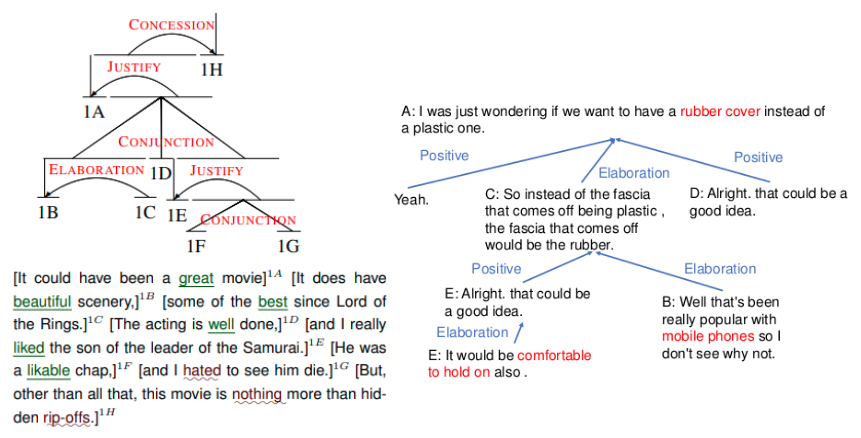
\includegraphics[width=1.0\columnwidth]{Images/dis_intro.png} 
  \caption{Left side: an example of RST discourse structure. Right side:  A meeting snippet. A, B, C, and E denotes different speakers. We show the attachment structure and the type of the speech act in blue.}
\end{figure}\label{fig:dis_intro} 

In this chapter, we study discourse in both spoken contexts and written texts, modeling discourse structures as latent variables. To fit into a machine learning framework, we will figure out ways to represent them as real value discrete random variable. Then we investigate the best model structure that can help us link the latent variable to the learning target, and estimate the value of the latent variable. We propose to use log-linear model, reinforcement learning, and sampling-based inference as our base models and learning methods. As we discussed earlier in section \ref{sec:ch-1}, latent information can be used to evaluate the performance of the model and make training process interpretable. We will demonstrate several ways to interpret prediction process by using latent information. Furthermore, we will show learned latent discourse structure can help us solve downstream tasks. Because discourse is not observable, we cannot feed it as numerical features to classifiers directly. We will rely on inference step of our model to build features based on its outputs.

In section \ref{sec:3-1}, we will first present a joint modeling approach to identify salient discussion points in spoken meetings as well as to label the discourse relations between speaker turns, and later, in section \ref{sec:3-2} we will show how discourse structure helps us generate interpretable reasoning paths in a reading comprehension task.


\section{Latent Discourse Relation in Extractive Text Summarization} \label{sec:3-1}


\begin{figure}[t]
\centering
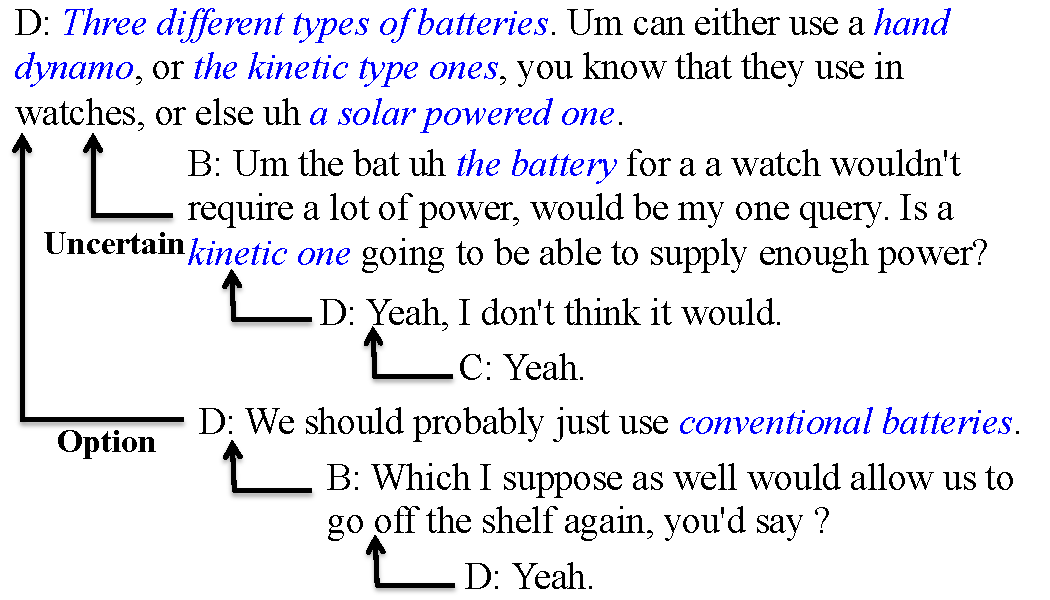
\includegraphics[width=98mm,height=60mm]{Images/snippet_intro.pdf}
%\vspace{-5mm}
\caption{ A sample clip from AMI meeting corpus. B, C, and D denotes different speakers. Here we highlight salient phrases (in \textit{italics}) that are relevant to the major topic discussed, i.e., ``which type of battery to use for the remote control''. Arrows indicate discourse structure between speaker turns. We also show some of the discourse relations for illustration.}
\label{fig:example_intro}
\end{figure}

\subsection{Background}

Goal-oriented dialogues, such as meetings, negotiations, or customer service transcripts, play an important role in our daily life. Automatically extracting the critical points and important outcomes from dialogues would facilitate generating summaries for complicated conversations, understanding the decision-making process of meetings, or analyzing the effectiveness of collaborations. In this work, we are interested in a specific type of dialogues --- spoken meetings, which is a common way for collaboration and idea sharing. Previous work~\cite{kirschner2012visualizing} has shown that discourse structure can be used to capture the main discussion points and arguments put forward during problem-solving and decision-making processes in meetings. Indeed, content of different speaker turns do not occur in isolation, and should be interpreted within the context of discourse. Meanwhile, content can also reflect the purpose of speaker turns, thus facilitate with discourse relation understanding. Take the meeting snippet from AMI corpus~\cite{ami} in Figure~\ref{fig:example_intro} as an example. This discussion is annotated with discourse structure based on the Twente Argumentation Schema (TAS) by Rutger~\cite{so65562}, which focuses on argumentative discourse information. As can be seen, meeting participants evaluate different options by showing doubt (\textsc{uncertain}), bringing up alternative solution (\textsc{option}), or giving feedback. The discourse information helps with the identification of the key discussion point, i.e., ``which type of battery to use'', by revealing the discussion flow.




% add some explanation for argumentative discourse
To date, most efforts to leverage discourse information to detect salient content from dialogues have focused on encoding gold-standard discourse relations as features for use in classifier training~\cite{murray2006incorporating,Galley:2006:SCR:1610075.1610126,mckeown2007using,Bui:2009:EDM:1708376.1708410}. However, automatic discourse parsing in dialogues is still a challenging problem~\cite{perret-EtAl:2016:N16-1}. Moreover, acquiring human annotation on discourse relations is a time-consuming and expensive process, and does not scale for large datasets. To avoid using labeled discourse features, it is natural to model discourse relation as latent variable, and use a joint modeling approach to select salient phrases reflecting key discussion points as well as label the discourse relations between speaker turns in spoken meetings. Specifically, we utilize argumentative discourse relations as defined in Twente Argument Schema (TAS)~\cite{so65562}, where discussions are organized into tree structures with discourse relations labeled between nodes (as shown in Figure~\ref{fig:example_intro}). Algorithms for joint learning and joint inference are proposed for our model. We also present a variation of our model to treat discourse relations as latent variables when true labels are not available for learning. We envision that the extracted salient phrases by our model can be used as input to abstractive meeting summarization systems~\cite{wang-cardie:2013:ACL2013,mehdad-carenini-ng:2014:P14-1}. Combined with the predicted discourse structure, a visualization tool can be exploited to display conversation flow to support intelligent meeting assistant systems.


\subsection{Jointly Modeling Content and Discourse Relations}

Our proposed model learns to jointly perform phrase-based content selection and discourse relation prediction by making use of the interaction between the two sources of information. 
%
Assume that a meeting discussion is denoted as $\mathbf{x}$, where $\mathbf{x}$ consists of a sequence of discourse units $\mathbf{x}=\{x_{1}, x_{2}, \cdots ,x_{n}\}$. Each discourse unit can be a complete speaker turn or a part of it. As demonstrated in Figure~\ref{fig:example_intro}, a tree-structured discourse diagram is constructed for each discussion with each discourse unit $x_{i}$ as a node of the tree. In this work, we consider the argumentative discourse structure by Twente Argument Schema (TAS)~\cite{so65562}. 
%
For each node $x_{i}$, it is attached to another node $x_{i^\prime}$ ($i^\prime<i$) in the discussion, and a discourse relation $d_{i}$ is hold on the link $\langle x_{i}, x_{i^\prime} \rangle$ ($d_{i}$ is empty if $x_{i}$ is the root). Let $\mathbf{t}$ denote the set of links $\langle x_{i}, x_{i^\prime} \rangle$ in $\mathbf{x}$.
%
Following previous work on discourse analysis in meetings~\cite{so65562,hakkani2009towards}, we assume that the attachment structure between discourse units are given during both training and testing. 


A set of candidate phrases are extracted from each discourse unit $x_{i}$, from which salient phrases that contain gist information will be identified. We obtain constituent and dependency parses for utterances using Stanford parser~\cite{Klein:2003:AUP:1075096.1075150}. We restrict eligible candidate to be a noun phrase (NP), verb phrase (VP), prepositional phrase (PP), or adjective phrase (ADJP) with at most 5 words, and its head word cannot be a stop word.\footnote{Other methods for mining candidate phrases, such as frequency-based method~\cite{liu2015mining}, will be studied for future work.} 
If a candidate is a parent of another candidate in the constituent parse tree, we will only keep the parent. We further merge a verb and a candidate noun phrase into one candidate if the later is the direct object or subject of the verb. For example, from utterance ``let's use a rubber case as well as rubber buttons'', we can identify candidates ``use a rubber case'' and ``rubber buttons''. 
For $x_{i}$, the set of candidate phrases are denoted as $c_{i}=\{c_{i,1},c_{i,2},\cdots,c_{i,m_i}\}$, where $m_i$ is the number of candidates. $c_{i,j}$ takes a value of $1$ if the corresponding candidate is selected as salient phrase; otherwise, $c_{i,j}$ is equal to $0$. All candidate phrases in discussion $\mathbf{x}$ are represented as $\mathbf{c}$.

%In this work, we focus on identifying salient phrases which contain gist information during a meeting, and predicting the discourse relations hold between discourse units. 

We then define a log-linear model with feature parameters $\mathbf{w}$ for the candidate phrases $\mathbf{c}$ and discourse relations $\mathbf{d}$ in $\mathbf{x}$ as:

%\vspace{-5mm}
{\fontsize{10}{10}\selectfont
\begin{equation}
\begin{split}
& p(\mathbf{c}, \mathbf{d}|\mathbf{x}, \mathbf{w}) \propto \exp [\mathbf{w}\cdot \Phi (\mathbf{c}, \mathbf{d}, \mathbf{x})] \propto \exp [\mathbf{w}\cdot \sum_{i=1, <x_i, x_{i^\prime}>\in \mathbf{t}}^{n} \phi (c_{i}, d_{i}, d_{i^\prime}, \mathbf{x})]\\
& \propto \exp [\sum_{i=1,<x_i, x_{i^\prime}>\in \mathbf{t}}^{n} ( \mathbf{w_c}\cdot \sum_{j=1}^{m_i} \phi_c (c_{i,j}, \mathbf{x})+ \mathbf{w_d}\cdot \phi_d (d_{i},d_{i^\prime}, \mathbf{x}) + \mathbf{w_{cd}}\cdot \sum_{j=1}^{m_i} \phi_{cd} (c_{i,j}, d_{i}, \mathbf{x}) ) ]\\
\end{split}
\end{equation}
\label{eq:objective}
}
%
Here $\Phi(\cdot)$ and $\phi(\cdot)$ denote feature vectors. We utilize three types of feature functions: (1) content-only features $\phi_c(\cdot)$, which capture the importance of phrases, (2) discourse-only features $\phi_d(\cdot)$, which characterize the (potentially higher-order) discourse relations, and (3) joint features of content and discourse $\phi_{cd}(\cdot)$, which model the interaction between the two. $\mathbf{w_c}$, $\mathbf{w_d}$, and $\mathbf{w_{cd}}$ are corresponding feature parameters. Detailed feature descriptions can be found in appendix \ref{sec:feature}. 

Acquiring labeled training data for discourse relations is a time-consuming process since it would require human annotators to inspect the full discussions. Therefore, we further propose a variation of our model where it treats the discourse relations as latent variables, so that $p(\mathbf{c} |\mathbf{x}, \mathbf{w})=\sum_{\mathbf{d}} p(\mathbf{c}, \mathbf{d}|\mathbf{x}, \mathbf{w})$. Its learning algorithm is slightly different as described latter. For learning the model parameters $\mathbf{w}$, we employ an algorithm based on SampleRank~\cite{rohanimanesh2011samplerank}, which is a stochastic structure learning method. In general, the learning algorithm constructs a sequence of configurations for sample labels as a Markov chain Monte Carlo (MCMC) chain based on a task-specific loss function, where stochastic gradients are distributed across the chain. %This is suitable for our learning problem because we aim to optimize the prediction performance for both phrase selection and discourse relations with various types of features.

The full learning procedure is described in Algorithm~\ref{alg:learning}. To start with, the feature weights $\mathbf{w}$ is initialized with each value randomly drawn from $[-1, 1]$. Multiple epochs are run through all samples. 
For each sample, we randomly initialize the assignment of candidate phrases labels $\mathbf{c}$ and discourse relations $\mathbf{d}$. 
%
Then an MCMC chain is constructed with a series of configurations $\sigma =(\mathbf{c}$, $\mathbf{d})$: at each step, it first samples a discourse structure $\mathbf{d}$ based on the proposal distribution $q(\mathbf{d^\prime} |\mathbf{d},\mathbf{x})$, and then samples phrase labels conditional on the new discourse relations and previous phrase labels based on $q(\mathbf{c^\prime} |\mathbf{c}, \mathbf{d^\prime},\mathbf{x})$. Local search is used for both proposal distributions.\footnote{For future work, we can explore other proposal distributions that utilize the conditional distribution of salient phrases given sampled discourse relations.}   
%
The new configuration is accepted if it improves on the score by $\omega (\sigma ^\prime)$. The parameters $\mathbf{w}$ are updated accordingly. For the scorer $\omega$, we use a weighted combination of F1 scores of phrase selection ($F1_{c}$) and discourse relation prediction ($F1_{d}$): $\omega (\sigma)= \alpha \cdot F1_{c} +  (1-\alpha) \cdot F1_{d}$. We fix $\alpha$ to $0.1$. When discourse relations are treated as latent, we initialize discourse relations for each sample with a label in $\{1, 2, \ldots, K\}$ if there are $K$ relations indicated, and we only use $F1_{c}$ as the scorer.
%We only use F1 score of phrase selection as our scorer.


\begin{algorithm}[t]
{
\SetKwInOut{Input}{Input}
\SetKwInOut{Output}{Output}

\Input{$\mathbf{X}=\{\mathbf{x}\}$: discussions in the training set, \\
	$\eta$: learning rate, 
	$\epsilon$: number of epochs, \\
	$\delta$: number of sampling rounds, \\
	$\omega (\cdot)$: scoring function,
	$\Phi (\cdot)$: feature functions
	}

\Output{feature weights $\frac{1}{|\mathcal{W}|}\sum_{\mathbf{w}\in \mathcal{W}} \mathbf{w}$}
\BlankLine

Initialize $\mathbf{w}$\;
$\mathcal{W} \leftarrow \{\mathbf{w} \}$\;

\For {$e=1$ to $\epsilon$} {

	\For {$\mathbf{x}$ in $\mathbf{X}$} {
	
		\tcp{Initialize configuration for $\mathbf{x}$}
		Initialize $\mathbf{c}$ and $\mathbf{d}$\;
		$\sigma=(\mathbf{c}, \mathbf{d})$\;
		\For {$s=1$ to $\delta$} {
			\tcp{New configuration via local search}
			$\mathbf{d^\prime} \sim q_d(\cdot | \mathbf{x}, \mathbf{d})$\;
			$\mathbf{c^\prime} \sim q_d(\cdot | \mathbf{x}, \mathbf{c}, \mathbf{d^\prime})$\;
			
			$\sigma^\prime=(\mathbf{c^\prime}, \mathbf{d^\prime})$\;
			
			$\sigma^+=\arg \max_{\tilde{\sigma} \in \{\sigma, \sigma^\prime \}} \omega (\tilde{\sigma}) $\;
			$\sigma^-=\arg \min_{\tilde{\sigma} \in \{\sigma, \sigma^\prime \}} \omega (\tilde{\sigma}) $\;		
			
			$\hat{\nabla}=\Phi (\sigma^+)- \Phi (\sigma^-)$\;
			$\Delta \omega= \omega (\sigma^+)- \omega (\sigma^-)$\; 

			\tcp{Update parameters}			
			\If {$\mathbf{w}\cdot \hat{\nabla} < \Delta \omega$ \& $\Delta \omega\neq 0$}{
				$\mathbf{w} \leftarrow \mathbf{w}+\eta \cdot \hat{\nabla}$\;
				Add $\mathbf{w}$ in $\mathcal{W}$\;
			}
			
			\tcp{Accept or reject new configuration}
			\If {$\sigma^+ == \sigma^\prime$}{
				$\sigma=\sigma^\prime$
			
			}
		}
	
	}
}
}

\caption{\fontsize{10}{12}\selectfont  SampleRank-based joint learning.}
\label{alg:learning}
\end{algorithm}

Given a new sample $\mathbf{x}$ and learned parameters $\mathbf{w}$, we predict phrase labels and discourse relations as $\arg \max_{\mathbf{c}, \mathbf{d}} p(\mathbf{c}, \mathbf{d}|\mathbf{x}, \mathbf{w})$. Dynamic programming can be employed to carry out joint inference, however, it would be time-consuming since our objective function has a large search space for both content and discourse labels. Hence we propose an alternating optimizing algorithm to search for $\mathbf{c}$ and $\mathbf{d}$ iteratively. Concretely, for each iteration, we first optimize on $\mathbf{d}$ by maximizing $\sum_{i=1,<x_i, x_i^\prime>\in \mathbf{t}}^{n} (\mathbf{w_d}\cdot \phi_d (d_{i},d_{i^\prime}, \mathbf{x}) + \mathbf{w_{cd}}\cdot \sum_{j=1}^{m_i} \phi_{cd} (c_{i,j}, d_{i}, \mathbf{x}))$. Message-passing~\cite{smith2008dependency} is used to find the best $\mathbf{d}$.

In the second step, we search for $\mathbf{c}$ that maximizes $\sum_{i=1,<x_i, x_i^\prime>\in \mathbf{t}}^{n} (\mathbf{w_c}\cdot \sum_{j=1}^{m_i} \phi_c (c_{i,j}, \mathbf{x}) + \mathbf{w_{cd}}\cdot \sum_{j=1}^{m_i} \phi_{cd} (c_{i,j}, d_{i}, \mathbf{x}) )$. We believe that candidate phrases based on the same concepts should have the same predicted label. Therefore, candidates of the same phrase type and sharing the same head word are grouped into one cluster. We then cast our task as an integer linear programming problem.\footnote{We use lpsolve: \url{http://lpsolve.sourceforge.net/5.5/}.} We optimize our objective function under constraints: (1) $c_{i,j}=c_{i^\prime, j^\prime}$ if $c_{i,j}$ and $c_{i^\prime, j^\prime}$ are in the same cluster, and (2) $c_{i,j}\in \{0, 1\} $, $\forall i, j$. The inference process is the same for models trained with latent discourse relations.

We evaluate our joint model on the AMI meeting corpus~\cite{ami}, where consists of 139 scenario-driven meetings and labeled with gold-standard discourse relations and summaries. Two variations of our joint model are tested: one is trained on gold-standard discourse relations, the other is trained by treating discourse relations as latent variables, and these two  methods are henceforth referred as \textit{Our Model} and \textit{Our Model-latent}. 

We evaluate whether the prediction of the content selection component can be used for summarizing the key points on discussion level. For each discussion, salient phrases identified by our model are concatenated in sequence for use as the summary. We consider two types of gold-standard summaries. One is utterance-level extractive summary, which consists of human labeled summary-worthy utterances. The other is abstractive summary, where we collect human abstract with at least one link from summary-worthy utterances.

\begin{table}[ht]

\parbox{.47\linewidth}{\fontsize{8}{9}\selectfont
\setlength{\tabcolsep}{0.8mm}
\begin{tabular}{|l|l|l|l|l|l|l|l|}

\hline

	\multicolumn{8}{|l|}{\textit{Extractive Summaries as Gold-Standard}}\\ \hline
    & &\multicolumn{3}{c|}{\textsc{ROUGE-1}} & \multicolumn{3}{c|}{\textsc{ROUGE-SU4}}\\ \hline
    & Len & Prec & Rec & F1 & Prec & Rec & F1\\ 
%   \underline{\textbf{Comparisons}} & & & & & & &  \\ 
	Longest DA & 30.9 & 64.4 & 15.0  & 23.1 & 58.6 & 9.3 & 15.3 \\ 
   	Centroid DA & 17.5 & {\bf 73.9} & 13.4 & 20.8 & {\bf 62.5} & 6.9 & 11.3 \\ 
	SVM & 49.8& 47.1 & 24.1 & 27.5 & 22.7 & 10.7 & 11.8 \\ 
    Liu \cite{liu2009unsupervised} & 62.4& 40.4 & 39.2 & 36.2 & 15.5 & 15.2 & 13.5 \\ 
    \hline\hline
	Our Model & 66.6 & 45.4 & 44.7 & 41.1$\ast$ & 24.1$\ast$ & 23.4$\ast$ & 20.9$\ast$ \\ 
   	Our Model-latent & 85.9 & 42.9 & {\bf 49.3} & {\bf 42.4}$\ast$ & 21.6 & {\bf 25.7}$\ast$ & {\bf 21.3}$\ast$ \\ 
   
 \hline\hline

	\multicolumn{8}{|l|}{\textit{Abstractive Summaries as Gold-Standard}}\\ \hline
    & &\multicolumn{3}{c|}{\textsc{ROUGE1}} & \multicolumn{3}{c|}{\textsc{ROUGE-SU4}}\\ \hline
    &  Len & Prec & Rec & F1 & Prec & Rec & F1\\ 
%   \underline{\textbf{Comparisons}} & & & & & & &  \\ 
	Longest DA & 30.9 & 14.8  & 5.5 & 7.4 & 4.8 & 1.4 & 1.9 \\ 
   	Centroid DA & 17.5 &{\bf 24.9} &  5.6 & 8.5 & {\bf 11.6} & 1.4 & 2.2 \\ 
   	SVM & 49.8& 13.3& 9.7  & 9.5 & 4.4 & 2.4 & 2.4 \\ 
    Liu \cite{liu2009unsupervised} & 62.4& 10.3 & 16.7 & 11.3 & 2.7 & 4.5 & 2.8 \\ 
    \hline\hline
    
	Our Model & 66.6& 12.6 & 18.9 & {\bf 13.1}$\ast$ & 3.8 & 5.5$\ast$ & {\bf 3.7}$\ast$ \\ 
	Our Model-latent & 85.9 & 11.4 & {\bf 20.0} & 12.4$\ast$ & 3.3 & {\bf 6.1}$\ast$ & 3.5$\ast$ \\ 
   
    \hline
\end{tabular}
\caption{\fontsize{10}{12}\selectfont ROUGE scores for phrase-based extractive summarization evaluated against human-constructed utterance-level extractive summaries and abstractive summaries. Our models that statistically significantly outperform SVM and Liu \cite{liu2009unsupervised} are highlighted with $\ast$ ($p < 0.05$, paired $t$-test). Best ROUGE score for each column is in \textbf{bold}.}
\label{tab:summ}
}
\hfill
\parbox{.50\linewidth}{
\centering
	{\fontsize{8}{9}\selectfont
    \setlength{\tabcolsep}{0.6mm}
%    \hspace{-2mm}
    \begin{tabular}{|p{75mm}|}
    \hline
	
	\textbf{Meeting Clip}: \\
	D: can we uh power a light in this? can we get a strong enough battery to power a light? \\
	A: um i think we could because the lcd panel requires power, and the lcd is a form of a light so that$\ldots$\\
	D: $\ldots$it's gonna have to have something high-tech about it and that's gonna take battery power$\ldots$ \\
	D: illuminate the buttons. yeah it glows.\\
	D: well m i'm thinking along the lines of you're you're in the dark watching a dvd and you um you find the thing in the dark and you go like this $\ldots$ oh where's the volume button in the dark, and uh y you just touch it $\ldots$ and it lights up or something.\\

	\hline \hline    
    
	\textbf{Abstract by Human}: \\
    What sort of battery to use. The industrial designer presented options for materials, components, and batteries and discussed the restrictions involved in using certain materials.\\
	
	\hline \hline
	
	\textbf{Longest DA}: \\
	well m i'm thinking along the lines of you're you're in the dark watching a dvd and you um you find the thing in the dark and you go like this.\\
	\textbf{Centroid DA}: \\
	can we uh power a light in this?\\

	\textbf{Our Method}: \\
	- power a light, a strong enough battery, \\
	- requires power, a form, \\
	- a really good battery, battery power, \\
	- illuminate the buttons, glows, \\
	- watching a dvd, the volume button, lights up or something\\	
    \hline
    \end{tabular}
    
    }
	\caption{\fontsize{10}{12}\selectfont Sample summaries output by different systems for a meeting clip from AMI corpus (less relevant utterances in between are removed). Salient phrases by our system output are displayed for each turn of the clip, with duplicated phrases removed for brevity. }%Our system summary captures argumentation process and important outcomes of the discussion.}
\label{fig:example_summary}
}
\end{table}




% metrics
We calculate scores based on ROUGE~\cite{Lin:2003:AES:1073445.1073465}, which is a popular tool for evaluating text summarization~\cite{gillick2009global,liu2010using}. ROUGE-1 (unigrams) and ROUGE-SU4 (skip-bigrams with at most 4 words in between) are used. 
%The ROUGE scores are computed by using official ROUOGE software with standard options.\footnote{ROUGE option: -n 4 -w 1.2 -m -2 4 -u -c 95 -r 1000 -f A -p 0.5 -t 0 -a -d} 
% baselines and comparison
Following previous work on meeting summarization~\cite{Riedhammer:2010:LSS:1837521.1837625,wang-cardie:2013:ACL2013}, we consider two dialogue act-level summarization baselines: (1) \textsc{longest DA} in each discussion is selected as the summary, and (2) \textsc{centroid DA}, the one with the highest TF-IDF similarity with all DAs in the discussion. 
%
We also compare with an unsupervised keyword extraction approach by Liu \cite{liu2009unsupervised}, where word importance is estimated by its TF-IDF score, POS tag, and the salience of its corresponding sentence. With the same candidate phrases as in our model, we extend Liu \cite{liu2009unsupervised} by scoring each phrase based on its average score of the words. Top phrases, with the same number of phrases output by our model, are included into the summaries. 
%
Finally, we compare with summaries consisting of salient phrases predicted by an SVM classifier trained with our content features.

From the results in Table~\ref{tab:summ}, we can see that phrase-based extractive summarization methods can yield better ROUGE scores for recall and F1 than baselines that extract the whole sentences. 
%
Meanwhile, our system significantly outperforms the SVM-based classifiers when evaluated on ROUGE recall and F1, while achieving comparable precision. Compared to Liu \cite{liu2009unsupervised}, our system also yields better results on all metrics.

Sample summaries by our model along with two baselines are displayed in Table~\ref{fig:example_summary}. Utterance-level extract-based baselines unavoidably contain disfluency and unnecessary details. Our phrase-based extractive summary is able to capture the key points from both the argumentation process and important outcomes of the conversation. This implies that our model output can be used as input for an abstractive summarization system. It can also facilitate the visualization of decision-making processes.



\subsection{Predicting Consistency of Understanding}
As discussed in previous work~\cite{mulder2002assessing,mercer2004sociocultural}, both content and discourse structure are critical for building shared understanding among discussants. 
In this section, we test whether our joint model can be utilized to predict the consistency among team members' understanding of their group decisions, which is defined as consistency of understanding (COU) in Kim \cite{kim2016improving}. This downstream task can also be used to evaluate the correctness of the generated discourse structures.%with an objective to develop intelligent systems that can suggest review of topics potentially resulting in inconsistent understandings among participants.

Kim \cite{kim2016improving} establish gold-standard COU labels on a portion of AMI discussions, by comparing participant summaries to determine whether participants report the same decisions. If all decision points are consistent, the associated topic discussion is labeled as \textit{consistent}; otherwise, the discussion is identified as \textit{inconsistent}. Their annotation covers a subset transcripts in the \textsc{AMI} dataset (we shall call it \textsc{AMI-sub}). Therefore, we run the prediction experiments on \textsc{AMI-sub} by using the same annotation. 
Out of total 129 discussions in \textsc{AMI-sub}, 86 discussions are labeled as consistent and 43 are inconsistent. 

We construct three types of features by using our model's predicted labels. Firstly, we learn two versions of our model based on the ``consistent'' discussions and the ``inconsistent'' ones in the training set, with learned parameters $\mathbf{w_{con}}$ and $\mathbf{w_{incon}}$. For a discussion in the test set, these two models output two probabilities $p_{con}=\max_{\mathbf{c}, \mathbf{d}} P(\mathbf{c}, \mathbf{d}|\mathbf{x}, \mathbf{w_{con}})$ and $p_{incon}=\max_{\mathbf{c}, \mathbf{d}} P(\mathbf{c}, \mathbf{d}|\mathbf{x}, \mathbf{w_{incon}})$. We use $p_{con}-p_{incon}$ as a feature. Furthermore, we consider discourse relations of length one and two from the discourse structure tree. Intuitively, some discourse relations, e.g., \textsc{elaboration} followed by multiple \textsc{positive} feedback, imply consistent understanding. The third feature is based on word entrainment, which has been shown to correlate with task success for groups~\cite{nenkova2008high}. Using the formula in Nenkova~\cite{nenkova2008high}, we compute the average word entrainment between the main speaker who utters the most words and all the other participants. The content words in the salient phrases predicted by our model is considered for entrainment computation.


\begin{table}[t]
\centering
\fontsize{9}{10}\selectfont
%\setlength{\baselineskip}{0pt}
\setlength{\tabcolsep}{1.5mm}
\begin{tabular}{|l|c|c|}
    \hline
%         &\multicolumn{2}{c|}{\textbf{SVM}}\\ 
        & \textbf{Acc} & \textbf{F1} \\ \hline
        \underline{\textbf{Comparisons}} && \\
        Baseline (Majority) & 66.7 & 40.0  \\ 
%        Baseline (Random) & 50.0 & 32.3\\ 
        Ngrams (SVM) & 51.2 & 50.6  \\ 
        %Kim \& Shah & 60.5 & 50.5 \\ \hline\hline
		Kim \cite{kim2016improving} & 60.5 & 50.5 \\ \hline\hline
		        
        \underline{\textbf{Features from Our Model}}&&  \\ 
        Consistency Probability (Prob) & 52.7 & 52.1 \\ 
        Discourse Relation (Disc) & 63.6 & 57.1$\ast$  \\ 
        Word Entrainment (Ent) & 60.5$\ast$ & 57.1$\ast$\\ 
        Prob + Disc+ Ent & {\bf 68.2}$\ast$ & {\bf 63.1}$\ast$  \\ \hline\hline

        \underline{\textbf{Oracles}}&&  \\ 
        Discourse Relation & 69.8 & 62.7 \\ 
        Word Entrainment & 61.2 & 57.8 \\ \hline
\end{tabular}
\caption{Consistency of Understanding (COU) prediction results on \textsc{AMI-sub}. Results that statistically significantly outperform ngrams-based baseline and Kim \cite{kim2016improving} are highlighted with $\ast$ ($p < 0.05$, paired $t$-test). %Best result (excluding oracles) for each column is in \textbf{bold}. 
For reference, we also show the prediction performance based on gold-standard discourse relations and phrase selection labels.}
\label{tab:consistency}
\end{table}

\noindent \textbf{Results.} 
Leave-one-out is used for experiments. For training, our features are constructed from gold-standard phrase and discourse labels. Predicted labels by our model is used for constructing features during testing. SVM-based classifier is used for experimenting with different sets of features output by our model. 
A majority class baseline is constructed as well. We also consider an SVM classifier trained with ngram features (unigrams and bigrams). Finally, we compare with the state-of-the-art method in Kim ~\cite{kim2016improving}, where discourse-relevant features and head gesture features are utilized in Hidden Markov Models to predict the consistency label.

The results are displayed in Table~\ref{tab:consistency}. All SVMs trained with our features surpass the ngrams-based baseline. Especially, the discourse features, word entrainment feature, and the combination of the three, all significantly outperform the state-of-the-art system by Kim \cite{kim2016improving}.\footnote{We also experiment with other popular classifiers, e.g. logistic regression or decision tree, and similar trend is respected.}




\section{Latent Discourse Marker Guided Reasoning Path in Text based Question Answering} \label{sec:3-2}

\subsection{Background}
Reading comprehension (RC) tasks have gained lots of attention from NLP research community during the past few years.  Two types of RC tasks are widely studied: the extractive question answering task \cite{DBLP:conf/emnlp/RajpurkarZLL16,DBLP:conf/acl/RajpurkarJL18}, and the  multiple-choice question answering task \cite{DBLP:conf/aaai/AydinYLLGD14,DBLP:conf/aaai/KhashabiKSR18}. Most of the current state-of-the-art methods use deep neural networks (DNN) based structures to tackle these two tasks and achieve practical performance on a variety of RC datasets. The most recent DNN based model BERT \cite{DBLP:journals/corr/abs-1810-04805} has even outperformed human's performance on the SQuAD dataset \cite{DBLP:conf/emnlp/RajpurkarZLL16}. 
\begin{figure}[ht]
\centering
	{\fontsize{9}{10}\selectfont
    \setlength{\tabcolsep}{0.6mm}
%    \hspace{-2mm}
    \begin{tabular}{|p{75mm}|}
    \hline
\textbf{Context: }\textit{\textcolor{red}{After}} inflation stopped, \textit{\textcolor{blue}{reheating }}occurred \textit{\textcolor{red}{until}} the universe obtained the temperatures required for the production of a quark-gluon plasma \textit{\textcolor{red}{as well as}} all other elementary particles. \\
\textbf{Question: }When did \textit{\textcolor{blue}{reheating}} stop?     \\
\textcolor{gray}{(reasoning step 1: focus on the context to the right of ``until'')}\\
\textbf{Context: }the universe obtained the temperatures required for the production of a quark-gluon plasma \textit{\textcolor{red}{as well as}} all other elementary particles. \\
\textcolor{gray}{(reasoning step 2: focus on the context to the left of ``as well as'')}\\
\textbf{Answer: }until the universe obtained the temperatures required for the production of a quark-gluon plasma \\
\hline
    \end{tabular}
    }
\caption{An Example in QAMR: The words in italics are discourse markers (in red) and question topic words (in blue). Reasoning steps are highlighted in gray. }
\label{fig:qa_example}
\end{figure}

Most existing deep learning models are either deep structures without internal steps, or with internal steps that do not justify comprehension. In other words, these models generate answers directly without giving human-understandable reasoning of the answer. Another disadvantage of the end-to-end DNN models is that the model is only valid for a specific domain of the training data, that is, the knowledge is not transferable to datasets in other domains. %Also, the knowledge are not explainable or interpretable as reasoning (by users). 
By contrast, humans can answer questions following reasoning steps which are reproducible and transferable.  

To address these issues, we introduce a novel deep reasoning model for RC tasks, by taking advantage of the discourse information in the context. The model design is inspired by the reading behavior of a well trained reader (``mature reader''). A human reader would not search for the answer by simply reading the entire document without any focus. Instead he will look for the answer based on question topics and discourse markers ( \emph{e.g.} ``however'' and ``because'')~\cite{assiri2011test,sungatullina2016metacognitive}. Question topics and discourse markers can help the reader quickly select the most relevant segments (pieces of text) to read, and skip those less relevant ones. Figure \ref{fig:qa_example} gives an example on how a ``mature reader'' finds an answer to a given question in a context paragraph. First, by reading the question, the reader notices the topic word ``reheating'' and the question type ``when-''. Then the reader searches for words that indicate \emph{time} from the given context, which could be ``after'' or ``until''. By analyzing the relationship between these time indicators and the target word ``reheating'', the reader focuses on the context after ``until''. Next, the reader splits the current focus by the connective ``as well as'' into two clauses, which are complementary to each other. Finally, the reader picks the text segment between ``until'' and ``as well as'' as the final answer. In this way, we define a reasoning path as a sequence of binary selections based on discourse markers. In the next section, we will show how to model such a reasoning path as latent variable using reinforcement learning.


\subsection{An Interpretable Discourse Guided Deep Reasoning Model}

We propose a deep reasoning model (DRM) with an architecture as shown in Figure \ref{fig:systemDiagram}. The model has three components: the state generation module (SGM) implemented with two convolutional neural networks; the reasoning generation module (RGM) implemented as deep reinforcement learning via an actor-critic algorithm; and a context selection operator (CSO) that shrinks the text context given a discourse marker and a direction (left=before; right=after).


\begin{figure}
\centering
\begin{minipage}{.45\textwidth}
 \centering
 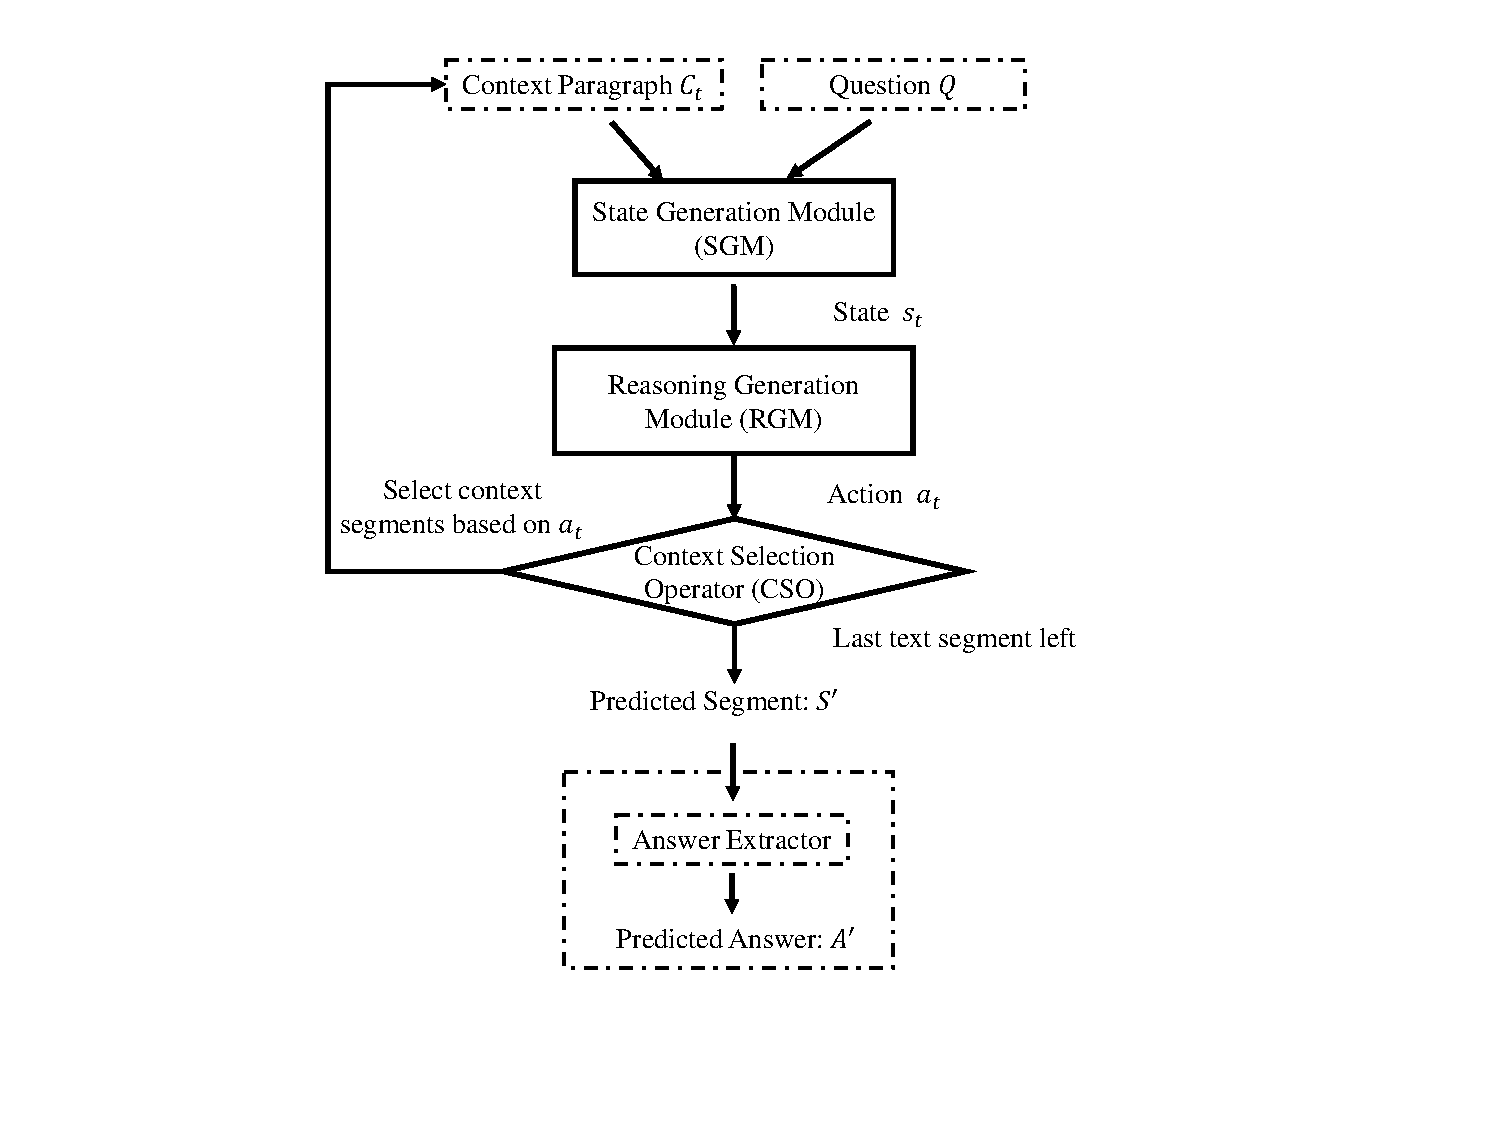
\includegraphics[width=0.9\linewidth]{Images/fig1.pdf}
 \caption{System Diagram}
 \label{fig:systemDiagram}
\end{minipage}
\end{figure}
%[Yu] \kechen{basic idea of RL and insight of using RL, multi step decision is naturally modeled by MDP}
% \subsection{Model Component Overview}
\label{sec2description}
The goal of our system is to mimic human reading behavior to extract a segment that
contains the answer. The mechanic in reducing the text context is analogous to binary search: Let $D=(D^1,D^2,...,D^k)$ be a list of discourse markers that appears in a context paragraph $C$. These discourse markers, working as the candidate partition points, divide the context into a list of segments $S=(S^1,S^2,...,S^{k+1})$. Then the context can be represented by a mixture of discourse markers and segments, $C=(S^1, D^1, S^2, D^2,...,D^k, S^{k+1})$. To identify the correct segment $S^*$ from $S$, our model at time-step $t$ works as follows:\\
(a) SGM encodes the context $C_t$ and question $Q$ into a vector representation, \emph{i.e.} the state $s_t$.\\
(b) RGM takes the state $s_t$ as its input, and predicts the partition point $D^{p(s_t)}_t$ (${p(s_t)}$ is the index selected at \emph{t}) and the reading focus $f_t \in \{left, right\}$. An action is defined as $a_t=(D^{p(s_t)}_t,f_t)$. \\
(c) CSO divides $C_t$ into two parts from $D^{p(s_t)}_t$: $C^1_t=(S^1, D^1,...,D^{p(s_t)-1}, S^{p(s_t)})$ and $C^2_t=(S^{p(s_t)+1}, D^{p(s_t)+1},...,D^k, S^{k+1})$, and keeps $C_{t+1} \leftarrow C_{t}^{1}$ if $f_t$ is left or $C_{t+1} \leftarrow C_{t}^{2}$ if $f_t$ is right. \\
The iterations stop when the output only contains a single text segment enclosed by two neighbor discourse markers. Intermediate output $D^{p(s_t)}_t$ at each time-step constitutes a reasoning path $(D^{p(1)}_1,...,D^{p(s_t)}_t)$. We note that during the prediction procedure the context $C_t$ changes, while the question $Q$ not (see Algorithm \ref{segment_alg}).

% \emph{Remarks:}
It is possible to add an answer extractor following the text segment $S'$ for a final answer (dashed in Figure \ref{fig:systemDiagram}). Since this is not our paper's focus and many existing works have been done achieve decent performance \cite{DBLP:conf/ijcai/HuPHQW018}, so this module is not discussed here. %\cite{DBLP:conf/acl/WangYWCZ17,DBLP:journals/corr/abs-1804-09541,DBLP:conf/ijcai/HuPHQW018}. Since this is not our paper's focus, we do not discuss it here.\\


%Since our paper's focus is not on answer extraction, and many existing works have been done achieve decent performance \cite{DBLP:conf/acl/WangYWCZ17,DBLP:journals/corr/abs-1804-09541,DBLP:conf/ijcai/HuPHQW018}, so this module is not discussed in this paper.



\begin{algorithm}
  \SetKwInOut{Input}{Input}
  \SetKwInOut{Output}{Output}

 % \underline{function Euclid} $(a,b)$\;
  \Input{$C$: context, $Q$: question}
  \Output{Answer segment: a single text segment enclosed by two neighbor discourse markers}
  $t = 0$\\
  $C_0 \leftarrow C$\\
  % Initialize model parameters\\
  \While {$C_t$ contains more than one text segment}{
    %SGM encodes the context $C_t$ and question $Q$ into a vector representation $s_t$.\\
    $s_t = SGM(C_t, Q)$ // generate state\\
    $D^{p(s_t)}_t,f_t= RGM(s_t)$ // generate action\\ 
   % $a_t=(D^{p(s_t)}_t,f_t)$ // an action consists of partition point $D^{p(s_t)}$ and reading focus $f_t$\\
    $C^1_t, C^2_t = CSO(C_t, D^{p(s_t)}_t)$\\
    \uIf{$f_t==left$}{
    //$C^1_t=(S^1, D^1,...,D^{p(s_t)-1}, S^{p(s_t)})$\\
        $C_{t+1} \leftarrow C_{t}^{1}$ 
    }\Else{
    //$C^2_t=(S^{p(s_t)+1}, D^{p(s_t)+1},...,D^k, S^{k+1})$\\
        $C_{t+1} \leftarrow C_{t}^{2}$ 
    }
    $t = t + 1$
  }
  $S^* \leftarrow C_t$\\
  \Return{$S^*$}
  \caption{Identifying the correct answer segment from the context}
  \label{segment_alg}
\end{algorithm}

We leverage a deep reinforcement learning (DRL) based structure to implement the reasoning generation module introduced in the above section. 
For every given context-question pair, the dataset provides an answer. Although this answer can be used to evaluate the final output of any reasoning path, there is no ground truth to evaluate the performance of each intermediate reasoning step $D^{p(s_t)}_t$. There are usually several different reasoning paths leading to the correct answer segment, based on different sequences of selecting discourse markers; thus the  task of searching for the best path fits well into the reinforcement learning, as these actions can reasonably imitate the human actions.

\begin{table*}[t]

	\begin{center}
	\resizebox{1.0\columnwidth}{!}{%resize the table
		\begin{tabular}{|l|c|c|c|c|cccccccc|}
			\hline
       \textbf{Method} & \textbf{Loss} & \textbf{Discourse} & \textbf{Target Word} 
      & \textbf{All} & \textbf{What} & \textbf{Whose} & \textbf{How} & \textbf{Why} & \textbf{Where} & \textbf{Who} & \textbf{When} & \textbf{Which} \\

            \hline
      Gradient Boosting & binary & &
      & .488 & .485 & .523 & .502 & .461 & .477 & .471 & .517 & .561 \\
      Gradient Boosting & binary & \checkmark &\checkmark 
      & .673 & .676 & .633 & .664 & .538 & .659 & .662 & .721 & .684 \\
            Gradient Boosting & ranking & & 
      & .469 & .486 & .397 & .414 & .566 & .475 & .447 & .453 & .457 \\
      Gradient Boosting & ranking & \checkmark &\checkmark 
      & .670 & .673 & .638 & .657 & .538 & .657 & .662 & .721 & .684 \\
      BM25 & ranking & &
      & .536 & .545 & .679 & .543 & .160 & .529 & .510 & .464 & .594 \\

      Coarse-to-Fine Answer Selector & binary & &
      & .540 & .539 & .490 & .506 & \textbf{.615} & .524 & .552 & .571 & .558 \\
     % CNN & binary & &
     % & .511 & .508 & .528 & .515 & .564 & .496 & .513 & .517 & .522 \\
      RaSoR & multi-class & &
      & .615 & .620 & \textbf{.706} & .598 & .560 & .599 & .598 & .586 & .659 \\
      \hline
      DRM-noRL & binary & \checkmark & \checkmark 
       & .664 & .667 & .619 & .649 & .564 & .653 & .657 & .706 & .678 \\
      DRM-type 1 & RL & \checkmark & 
      & .691 & .696 & .676 & .681 & \textbf{.615} & .696 & .671 & .724 & .702 \\
      DRM-type 2 & RL & \checkmark & \checkmark 
      & \textbf{.702}  & \textbf{.703} & .676 & \textbf{.684} & \textbf{.615} & \textbf{.701} & \textbf{.677} & \textbf{.733} & \textbf{.705} \\
      DRM-type 2 w/ human & RL & \checkmark & \checkmark 
      & \textbf{.797} & \textbf{.801} & \textbf{.789} & \textbf{.769} & \textbf{.820} & \textbf{.778} & \textbf{.793} & \textbf{.815} & \textbf{.810} \\
      \hline

		\end{tabular}

				}\vspace{0.4mm}	\\
\small{Table 3(a): Results on QAMR-SUBSET dataset.}\\\vspace{2mm}
	\resizebox{1.0\columnwidth}{!}{%resize the table
		\begin{tabular}{|l|c|c|c|c|cccccccc|}
			\hline
       \textbf{Method} & \textbf{Loss} & \textbf{Discourse} & \textbf{Target Word} 
      & \textbf{All} & \textbf{What} & \textbf{Whose} & \textbf{How} & \textbf{Why} & \textbf{Where} & \textbf{Who} & \textbf{When} & \textbf{Which} \\

            \hline
      Gradient Boosting & binary & &
      & .338 & .355 & .363 & .289 & .166 & .291 & .311 & .263 & .428 \\
      Gradient Boosting & binary & \checkmark &\checkmark 
      & .575 & .586 & .528 & \textbf{.616} & .666 & .632 & \textbf{.621} & \textbf{.610} & \textbf{.528} \\
            Gradient Boosting & ranking & & 
      & .360 & .376 & .454 & .339 & .666 & .354 & .335 & .276 & .301 \\
      Gradient Boosting & ranking & \checkmark &\checkmark 
      & .561 & .567 & .424 & .578 & .166 & .583 & .566 & .539 & .507 \\
      BM25 & ranking & &
      & .456 & .481 & .380 & .393 & .0.0 & .448 & .439 & .444 & .491 \\

      Coarse-to-Fine Answer Selector & binary & &
      & .405 & .422 & .363 & .408 & .166 & .312 & .376 & .315 & .492 \\
      %CNN & binary & &
      %& .356 & .346 & .242 & .359 & .666 & .437 & .376 & .355 & .365 \\
      RaSoR & multi-class & &
      & .539 & .545 & \textbf{.619} & .525 & .375 & .528 & .552 & .487 & .491 \\
      \hline
      DRM-noRL & binary & \checkmark & \checkmark 
       & .573 & .571 & .606 & .591 & .833 & \textbf{.645} & .572 & .513 & .539 \\
      DRM-type 1 & RL & \checkmark & 
      & .569 & .579 & .515 & .572 & \textbf{.833} & .625 & .560 & .513 & .492 \\
      DRM-type 2 & RL & \checkmark & \checkmark 
      & \textbf{.599} & \textbf{.599} & .575 & \textbf{.616} & \textbf{.833} & \textbf{.666} & .598 & .565 & .523 \\
      DRM-type 2 w/ human & RL & \checkmark & \checkmark 
      & \textbf{.676} & \textbf{.676} & \textbf{.727} & \textbf{.683} & \textbf{1.0} & .500 & \textbf{.698} & \textbf{.618} & \textbf{.682} \\
      \hline
    
		\end{tabular}

		}\vspace{0.4mm}	\\

	\end{center}
	\caption{Comparison of different approaches. We show the training loss (binary: binary cross entropy loss, ranking: ranking loss, multi-class: cross entropy loss, RL: reinforcement learning loss in formula \ref{rlloss}.), and check whether discourse or target word is used in each method. We highlight the top scores of each column in bold. 
  }\label{tab:main3}
\end{table*}

A typical reinforcement learning structure contains four main elements: the state ($s_t$), the action ($a_t$), the reward ($r_t$), and the policy ($\pi$). In general, by taking an action $a_t$, a RL agent can move from its current state $s_t$ to another state $s_{t+1}$ and receive a reward $r_t$. The final target of a RL model is to learn an optimal policy $\pi$ such that the system can maximize the expected total reward $R_t=\mathop{\mathbb{E}}_\pi[\sum_{t=0}^{T}\gamma^t r_t]$ obtained at each state $s_t$, where $s_T$ is the final state. Specifically in our problem, at each time-step $t$ our model is in state $s_t$ containing the information of the current context $C_t$ and the question $Q$; it takes action $a_t$ choosing the appropriate discourse marker and the direction (reading focus) in order to maximize the expected reward $R_t$. We consider two types of actions with/without using labeled question topic, and name them DRM-type 1 and DRM-type 2. More details of the RL configurations can be found in appendix \ref{sec:design}.

This study uses two corpora from Question-Answer Meaning Representations datasets \cite{DBLP:conf/naacl/MichaelSHDZ18}: the QAMR corpus and the PTB corpus. The QAMR corpus consists of 69,320 QA pairs for 4,238 context paragraphs extracted from Wikipedia, and the PTB corpus consists of 27,082 QA pairs for 253 context paragraphs extracted from Penn Treebank \cite{DBLP:journals/coling/MarcusSM94}. A target word, which appears in the question and represent the question topic is associated with each QA pair in the datasets. We report the overall segment prediction accuracy on the datasets and the accuracy on each question type (Table~\ref{tab:main3}). Descriptions of baseline methods can be found in appendix \ref{qa_baseline}. On both QAMR dataset and PTB dataset, DRM-type 2 with human in the loop achieves the highest accuracy. Being able to interact with humans is an advantage of our approach; 
% Humans can understand the decision process of the algorithm and can intervene if necessary. By contrast, 
none of the competitor approaches can do this, either because their decision process is a single-step process or because their decision process is not interpretable. In our experiment, 65\% QA pairs (less than the threshold) get help from human at one reasoning step, and their performance increases 0.15. It is also very interesting to learn that the remaining 35\% data points with high confidence reasoning learned by our model perform 0.06 better than the average performance. To further understand whether the improvement comes from human's selection or from our model's judgement, we allow the model to randomly select 65\% of the QA pairs, and for each pair, to interact with human once without considering their confidence. The results show that such random selection procedure doesn't make any difference on performance. Even without human's help, our DRM-type 2 model still achieves better performance than all other methods. As expected, DRM-type 2 model performs better than DRM-type 1 model, since type 2 actions leverage more information. 
%Looking at how the algorithm performs as the number of reasoning steps increases, the prediction accuracy increases slightly as the reasoning gets longer: the accuracy for 1-step, 2-step, 3-step and 4-step reasoning is 0.700,0.700,0.705 and 0.727.

Among the baseline methods, Gradient Boosting trained on both bag-of-words + discourse features works best. These models perform much worse if trained only on bag-of-words features. This shows that the structure/order information captured by discourse features is essential, which Neural network doesn't do. 
% The classical BM25 works well on questions that start with ``whose" but terribly on questions that start with ``why". 
Since BM25 solely relies on similarity between the question and the segment, it only works well when the the question and the correct segment have many overlapping words, as in the case of ``whose'' questions, but not ``why'' questions.

%0. RL learning curve\\




\begin{table*}[t]
\centering
{
	\fontsize{9}{9}\selectfont
  %\setlength{\baselineskip}{0pt}
  \setlength{\tabcolsep}{1.0mm}
  \renewcommand{\arraystretch}{1.1}
	%\hspace{4mm}
	\begin{tabular}{|p{1.8cm}|p{2.5cm}|p{2.5cm}|p{2.5cm}|p{5.8cm}|}
 	\hline
 	\textbf{Question genre}  & \textbf{Same side}& \textbf{Opposite sides}& \textbf{Context-dependent (side)} &  \textbf{Example QA pairs} \\
 	\hline
 	when \newline what year \newline how long 
 	& \textbf{step 1}: already, again, still, following \newline\textbf{step 2}: while, yet & \textbf{step 1}: as soon as, at that \newline\newline \textbf{step 2}: then, further, originally
 	&\textbf{step 1}: previously, until, back, after, soon, during \newline \textbf{step 2}: since, second, next, when, as well, because, who 
	&  \textbf{Context: }28 \textit{\textcolor{blue}{skiers}} earned DNFs \textit{\textcolor{red}{during}} \underline{the first run}, \textit{\textcolor{red}{and}} nine earned DNFs \textit{\textcolor{red}{during}} their second runs.
  \newline \textbf{Question: }When did \textit{\textcolor{blue}{skiers}} earn DNFs? 
  \newline \textbf{Learned Reasoning: } during-right, and-left\\ 
	\hline
  why \newline what caused 
 &\textbf{step 1}: in order to, because, due to,  since \newline\textbf{step 2}: as, but &\textbf{step 1}: at that, previously, though, if, since \newline \textbf{step 2}: second, for, to, or, that, not, and & \textbf{step 1}: well, following, initially  \newline\newline\textbf{step 2}: which, even,certainly  
  & \textbf{Context: }Given its initial condition, prediction of its final condition is possible, causally \textit{\textcolor{red}{but}} only probabilistically, \textit{\textcolor{red}{because}} the Schrödinger equation is deterministic for wave function evolution, \textit{\textcolor{red}{but}} \underline{the wave function describes the system only} \underline{\textit{\textcolor{blue}{probabilistically}}}.
  \newline \textbf{Question: }Why is the prediction \textit{\textcolor{blue}{probabilistic}}?
  \newline \textbf{Learned Reasoning: }because-right, but-right\\ 
	\hline	
	who+past tense 

	& \textbf{step 1}: rather, thus, including \newline\newline\textbf{step 2}: nor, who, initially &\textbf{step 1}: earlier, definitely, previously \newline\newline\textbf{step 2}: particularly, seemingly
		&\textbf{step 1}: ultimately, since, when, later, while, finally \newline \textbf{step 2}:  again, last, and , after, next, 
	& \textbf{Context: }\underline{Hatch had} \textit{\textcolor{red}{previously}} \textit{\textcolor{blue}{survived}} a separate crash in 2003, \textit{\textcolor{red}{that}} killed his mother, brother \textit{\textcolor{red}{and}} sister.
  \newline \textbf{Question: }Who \textit{\textcolor{blue}{survived}}?\newline \textbf{Learned Reasoning: }previously-left\\ 
	\hline
  where 
 
  
	 &\textbf{step 1}: following, to explain, while \newline\newline\textbf{step 2}: possibly, initially, finally, hence &\textbf{step 1}: to, before, back, in that, eventually \newline\textbf{step 2}: like, or, as & \textbf{step 1}: in which, then, second, next \newline\newline \textbf{step 2}: too, yet, second, including, after, next
  & \textbf{Context: }\textit{\textcolor{red}{Once}} the proposed \textit{\textcolor{blue}{amendment}} has passed those hurdles, \textit{\textcolor{red}{then}} the amendment goes \textit{\textcolor{red}{to}} \underline{Indiana voters} \textit{\textcolor{red}{who}} vote yea or nay on the amendment. 
  \newline \textbf{Question: }Where does the \textit{\textcolor{blue}{amendment}} go?
  \newline \textbf{Learned Reasoning: }to-right, who-left\\ 
 \hline
\end{tabular}
}
\caption{Top discourse markers are associated with question genres, and focus direction is learned in \textsc{QAMR-SUBSET} dataset. We show four different question genres: time, reason, person, and location.}
\label{tab:disc_phrase}
\end{table*}

\section{Proposed work}

In the question answering task, we have developed a QA system that attempts to generate both final answer and the interpretable reasoning path, and evaluated the performance of answer generation. How to evaluate the interpretability of the system would be a natural follow up work. Since there is no direct way to evaluate reasoning chains, we propose to use human identification and run proxy tasks instead. 


\subsection{Reasoning with Human Identification} \label{future_reason}


We first propose to evaluate generated reasoning path with human identification. The goal is to inspect the trained model and find the discourse markers which have the greatest impact for each question type. In a preliminary study, we show a few samples with the discourse markers used in the first two reasoning steps in Table~\ref{tab:disc_phrase}. As we can see, our model tends to rely on different discourse markers in different reasoning steps. The discourse markers used in the first step are quite tailored to the question type while those in the second step are only loosely related. This shows that our model can navigate to the most relevant discourse marker very quickly, typically within one step. Next we want to analyze how the model chooses the focus to move based on discourse markers and the location of the target word for type 2 action. From the second to the fourth columns in Table~\ref{tab:disc_phrase} we show which direction the model should move to at each discourse marker. For instance, to answer a ``why'' question, if the current discourse marker we are looking at is ``due to'', then the model expects the target word and the explanation part (the answer we are looking for) to appear on opposite sides of the marker, which matches our intuition (\textit{i.e.} \textit{target word} due to \textit{answer}). The fourth column shows some discourse markers depend on context to select side to focus. This preliminary results give us positive signals and motivate us to further design human identification methods to look into the reasoning process generated by the model.

\subsection{Reasoning with Downstream tasks}

In the text summarization work, we manage to evaluate the generated latent discourse structure by utilizing them in a consistency prediction task. Similarly, we would like to evaluate the generated reasoning path in a downstream task. For example, we can apply the deep reasoning model (DRM) to the task of understanding the persuasive essay. %Specifically, we aim to extract the major claims from an essay dataset by leveraging the knowledge encoded by DRM which was trained on a different dataset.  
Argument mining tasks include finding a sentence in an essay that can serve as the major claim and identifying its support arguments \cite{DBLP:conf/lrec/ReedPRM08}. Previous work \cite{DBLP:conf/emnlp/StabG14} has shown that both content and discourse are critical for understanding argument structures. Claims in persuasive essays heavily rely on the phrases that signal beliefs (\emph{e.g.} ``in my opinion'').  \cite{DBLP:conf/coling/StabG14} establishes gold-standard argument structure labels on a corpus of 90 persuasive essays. Each of these essays is associated with a topic, for instance \textit{``government and education''}. 

\textbf{Major claim extraction task.} In each essay, one clause is labeled as a major claim, for example \textit{``government should pay for the university fees''}. Other clauses are labeled with support or non-support to the major claim, for example a supportive argument is \textit{``Students would be able to focus more on their studies rather than worrying about how to scrape together enough funds for each upcoming school term.''}. We can ask our DRM model, trained on the question answering dataset~\textsc{QAMR-SUBSET}, to take a short paragraph and a question as inputs, and predict a short text segment as the output. A whole essay might be too long for the DRM, but on this dataset the major claim always appear in the first paragraph, so we can only feed the first paragraph of the essay, together with a made-up question concatenating \textit{``What is the opinion on''} to the essay's topic. For example, a question like \textit{``What is the opinion on government and education?''}. We then take the output segment of the DRM model and find the corresponding clause by highest overlap (essays are given segmented into clauses). We can compare the accuracy of the prediction with state-of-the-art results \cite{DBLP:conf/emnlp/StabG14}. In addition, we also want to see if our model can find the most indicative discourse markers of the major claims, such as ``that'' (\emph{e.g.} ``I strongly believe that...''), ``however'', ``therefore'', etc.

% We try to keep the extracted major claim sentence as complete as possible by discarding certain discourse markers (\emph{e.g.} ``to") that may split a sentence into multiple short phrases. We note, however, our solution is not perfect, and some major claim sentences are still not kept complete. %It also makes sure that the correct major claim would not be split into multiple phrases by discourse markers. %After these filtering, we find that 74 out of 90 essays contain a complete major claim. For the rest of essays, we still consider them in our test dataset, and we will show more details about prediction results below.
%We apply the trained DRM to all 90 essays in this dataset. For comparison, we take the SVM-based classifier proposed in \cite{DBLP:conf/emnlp/StabG14}, trained on many linguistic features. Our DRM outperforms the SVM method in terms of accuracy (0.489 \emph{vs.} 0.422). In particular, the DRM finds the most indicative of the major claims discourse markers  are: ``that'' (\emph{e.g.} ``I strongly believe that...''), ``however'', ``therefore'', etc.

\textbf{Support classification task.}  Furthermore, we want to test whether the model's predictions can be utilized to predict the argumentative relations between clauses and the major claim (support vs. non-support). We will design a set of features based on learned reasoning path, such as: (1) whether the clause contains discourse markers on the path to identifying the major claim; (2) whether the clause is on the same side with the final segment after the first selection by using DRM model. Intuitively, the reasoning path learned by DRM model implies support relations. After collecting new features, we will concatenate them to the existing linguistic binary features extracted by \cite{DBLP:conf/emnlp/StabG14}, and we expect to see an improvement on model performance by using our DRM features.







 
\chapter{Timeline} \label{ch-4}

\begin{table}[ht]
\resizebox{1.0\columnwidth}{!}{
\begin{tabular}{|l|l|l|l|}
\hline
 Timeline & Task &  Reference &Progress \\ \hline
 by June 2020 & Reasoning evaluation experiments for QA task &Section \ref{future_reason} & ongoing \\
 & - Human identification experiment&&\\
 & - Major claim extraction experiment&&\\
 & - Discourse relation classification experiment&&\\
 \hline
 by Winter 2020 & Improving path selection method &Section \ref{future_path} & planning \\
 & - Use current trained model to select good paths&&\\
 & - Use advanced bootstrapping methods to select good paths&&\\
 & - Figure out other ways to solve the problem&&\\
\hline
 by Winter 2020 & Improving model architecture &Section \ref{future_model} & planning \\
 & - Neural Transformer experiments&&\\
 & - Memory Network experiments&&\\
 & - Propose novel model structures&&\\
\hline
 by Summer 2021 & Handling noisy tags in multi-label classification &Section \ref{future_noise} & planning \\ 
 & - Propose novel ideas to handle noisy tags&&\\
 & - Propose novel model structures&&\\
\hline 
 by Fall 2021 & Thesis writing and defense. & All Sections & planning\\
 \hline
\end{tabular}
}
\end{table} 
 
%----------------------------------------------------------------------------------------
%	APPENDICES
%----------------------------------------------------------------------------------------

\addtocontents{toc}{\vspace{2em}} % Add a gap in the Contents, for aesthetics
\appendix % Starts of appendices

%----------------------------------------------------------------------------------------
%	BIBLIOGRAPHY
%----------------------------------------------------------------------------------------

\addtocontents{toc}{\vspace{2em}} % Add a gap in the Contents, for aesthetics
\unnumberedchapter{Bibliography} % Title of the unnumbered chapter
% \bibliographystyle{plainnat}
\bibliography{Preamble/Thesis_bibliography} % The references information are stored in the file named "Thesis_bibliography.bib"

\numberedchapter
\chapter{Baselines in Multi-label Prediction Experiment} \label{multi-baseline}

We compare our method with the following methods: 
\begin{itemize}
	\item \textbf{Binary Relevance (BR)} \cite{tsoumakas2007multi} with both independent training and prediction;
	\item \textbf{Binary Relevance with support inference (BR-support)} \cite{wang2018pipeline} which trains binary classifiers independently but imposes label constraints at prediction time by only considering label sets observed during training, namely $\hat{\mathbf{y}}=\arg\max_{\text{observed~}\mathbf{y}}\prod_{\ell=1}^L p(y_{\ell}|x)$;
	\item \textbf{Probabilistic Classifier Chain (PCC)} \cite{DBLP:conf/icml/DembczynskiCH10} which transforms the multi-label classification task into a chain of binary classification problems. Predictions are made with Beam Search.
  \item \textbf{Sequence to Sequence RNN (seq2seq-RNN)} \cite{DBLP:conf/nips/NamMKF17} which maps each set to a sequence by decreasing label frequency and solves the multi-label task with an RNN designed for sequence prediction. 
  \item \textbf{Vinyals-RNN-uniform, Vinyals-RNN-sample, and Vinyals-RNN-max} are three variants of RNNs proposed by \cite{vinyals2015order}. They are trained with different objectives that correspond to different transformations between sets and sequences. Following the approach taken by \cite{vinyals2015order}, Vinyals-RNN-sample and Vinyals-RNN-max are initialized by Vinyals-RNN-uniform. We have also tested training Vinyals-RNN-max directly without having Vinyals-RNN-uniform as an initialization, and we name it as \textbf{Vinyals-RNN-max-direct}.
  \item \textbf{Sequence Generation Model (SGM)} \cite{DBLP:journals/corr/abs-1806-04822} which trains the RNN model similar to seq2seq-RNN but uses a new decoder structure that computes a weighted global embedding based on all labels as opposed to just the top one at each timestep.
\end{itemize}

In BR and PCC, logistic regressions with L1 and L2 regularizations are used as the underlying binary classifiers. seq2seq-RNN, PCC, and SGM rely on a particular label order. We adopt the decreasing label frequency order, which is the most popular choice.
\chapter{Features used in Extractive Text Summarization Experiment}
\label{sec:feature}
We use features that characterize content, discourse relations, and the combination of both.

\noindent \textbf{Content Features.} 
For modeling the salience of content, we calculate the minimum, maximum, and average of \texttt{TF-IDF} scores of words and \texttt{number of content words} in each phrase based on the intuition that important phrases tend to have more content words with high TF-IDF scores~\cite{FernandezFDAEP08}. We also consider whether the head word of the phrase has been \texttt{mentioned in preceding turn}, which implies the focus of a discussion. The \texttt{size of the cluster} each phrase belongs to is also included. 
\texttt{Number of POS tags} and \texttt{phrase types} are counted to characterize the syntactic structure. Previous work~\cite{wang-cardie:2012:SIGDIAL20122} has found that a discussion usually ends with decision-relevant information. We thus identify the \texttt{absolute and relative positions} of the turn containing the candidate phrase in the discussion. Finally, we record whether the candidate phrase is \texttt{uttered by the main speaker}, who speakers the most words in the discussion. 


\noindent \textbf{Discourse Features.} 
For each discourse unit, we collect the \texttt{dialogue act types} of the current unit and its parent node in discourse tree, whether there is any \texttt{adjacency pair} held between the two nodes~\cite{hakkani2009towards}, and the \texttt{Jaccard similarity} between them.
%
We record whether two turns are \texttt{uttered by the same speaker}, for example, \textsc{elaboration} is commonly observed between the turns from the same participant. 
%
We also calculate the \texttt{number of candidate phrases} based on the observation that \textsc{option} and \textsc{specialization} tend to contain more informative words than \textsc{positive} feedback. 
Length of the discourse unit is also relevant. Therefore, we compute the \texttt{time span} and \texttt{number of words}.  
To incorporate global structure features, we encode the \texttt{depth of the node} in the discourse tree and \texttt{the number of its siblings}. 
%
Finally, we include an \texttt{order-2 discourse relation} feature that encodes the relation between current discourse unit and its parent, and the relation between the parent and its grandparent if it exists. 


\noindent \textbf{Joint Features.} For modeling the interaction between content and discourse, the discourse relation is added to each content feature to compose a joint feature. For example, if candidate $c$ in discussion $x$ has a content feature $\phi_{[avg-TFIDF]} (c, \mathbf{x})$ with a value of $0.5$, and its discourse relation $d$ is \textsc{positive}, then the joint feature takes the form of $\phi_{[avg-TFIDF, Positive]} (c, d, \mathbf{x})=0.5$. 

\chapter{States, Actions, Rewards}\label{sec:design}

\begin{figure}\centering
\begin{minipage}{.45\textwidth}
 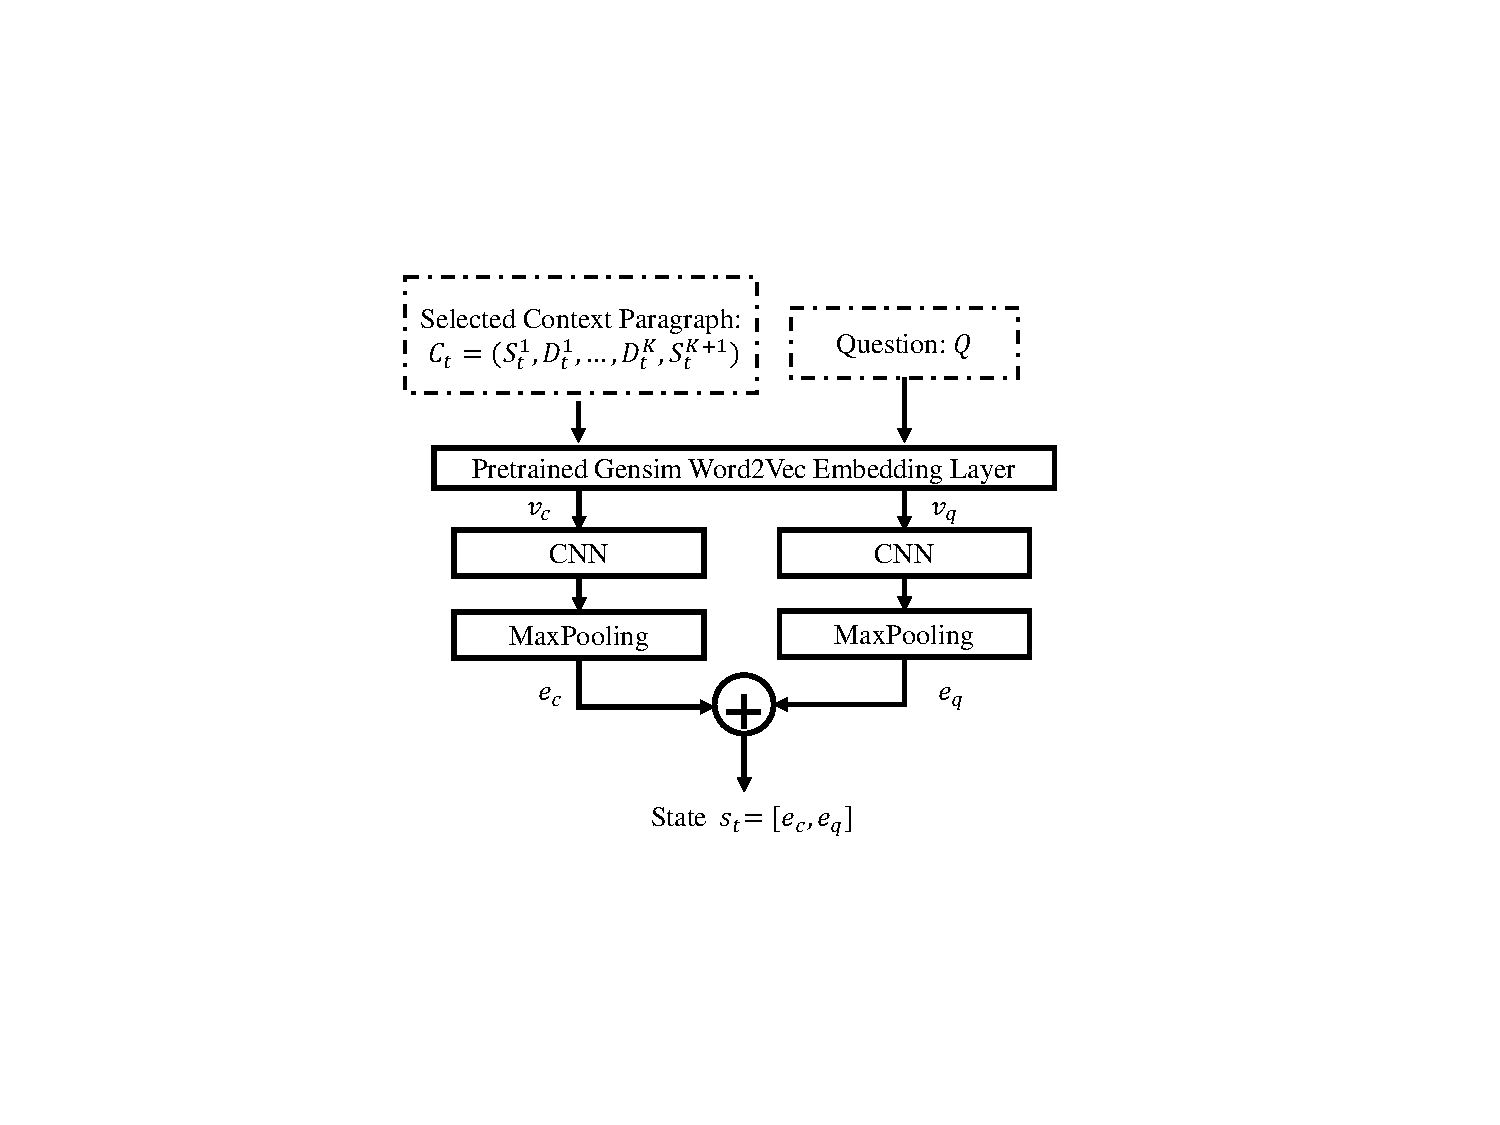
\includegraphics[width=0.9\linewidth]{Images/fig1_2.pdf}
 \caption{SGM Diagram}
 \label{fig:sgmDiagram}
\end{minipage}
\vspace{-2ex}
\end{figure}

\textbf{Design of State:} As our system's input, a state contains the information from both the context and the question (as shown in Figure \ref{fig:sgmDiagram}). %we designed state generation model (SGM) to generate their embeddings in order to construct the defined states. First, we train a preliminary word embedding dictionary using the gensim word2vec on a given dataset. By using these pre-trained word embeddings, 
We feed the context paragraph and the question separately into our state generation module (SGM), which contains an embedding layer and a convolutional layer followed by a max-pooling layer. The obtained embedding of the context paragraph is concatenated with that of the given question, in order to form a state as the input to RGM. The embedding layer is pre-trained using our dataset; the CNN and max-pooling layers are trained and updated together with our RL model. %, whose outputs are the actions to be defined in next section. Using this two-step approach, we can both leverage the fixed word-level information from our corpus and learn-able embedding information guided by the expected rewards obtained in DRL. %\kechen{add why we don't use coattention and intuition of choosing CNN}
%\subsection{Design of Actions}\label{design_action}
 %As defined in section XXX, t
 
 \textbf{Design of Actions:} The actions determine the reading focus at next time-step $t+1$. 
 % The design of actions is supposed to be close to one type of our human reasoning behaviors: using discourse markers and question topic to guide reading.
 Two different set of action designs are introduced as follows:
 
{\bf{ \underline{Action Set $1$:}}}
The first set of actions is designed only using the discourse markers, such that for each action, either context paragraph before or after a marker is chosen to be focused. An action is supposed to contain two pieces of information: (a) the word marker to be selected, and (b) the focus of reading from the selected marker, \emph{i.e. left} or \emph{right}. The action space is defined as $\lbrace\alpha_{1}^{left},\alpha_{1}^{right}, \cdots,\alpha_{k}^{left},\alpha_{k}^{right}\rbrace$, where $k$ discourse markers are selected from our discourse marker lexicon. The entire action space dimension is $\mathbb{R}^{2\times k}$ by considering the left and right directions. %After choosing an action, for example $\alpha_{i}^{left}$, the system will focus on the context \emph{left} to the discourse marker $d_{i}$, and vice versa for $\alpha_{i}^{right}$.

%\vspace{-1.0mm}
%\begin{itemize}[itemsep=0.1mm]
%\item The word marker to be selected.
%\item The focus of reading from the selected marker, \emph{i.e.} left or right.
%\vspace{-1.0mm}
%\end{itemize}
%In our model, we use the discourse marker, which is a main type of connectives, as the word markers described before. 

%which divide a document into multiple sentences/phrase segments. As in XXX, a human reader would like to use a word marker for reasoning in a machine reading task, %\cheng{I am not sure there is how humans read. I am not sure that the reviewers will buy this argument. Is there any behavior or psychological study that shows humans search for answers this way?} 
%Assuming that our system wants to imitate this learning process, our system's 
%Inspired by the work in XXX, in our model, we use the discourse markers, which is a main type of connectives, as the word markers for the model to select in this type of action design. 
%Furthermore, we also use the combination of discourse markers and target word(s) to define our action as shown in the second type of action design. \cheng{This is repeated in earlier sections}

%Also, in order to limit the action space size, we only select top $k$ discourse markers from XXX ranked by their frequencies in our datasets. By considering the searching directions from the selected discourse marker(s), the action space size is $2\times k$, which is the double of number of discourse markers selected. 
%A graphical illustration is as shown in Figure XXX:

%The action space includes $2\times k$ actions. At each time step $t$, the system selects one of them as the output of our DRL model. Specifically in our case, the DRL model will generate an action vector with a size of $2\times k$, where one of numbers in the vector is 1, and all the others are equal to 0s\kechen{why is that?}.


 {\bf{\underline{Action Set $2$:}}} The second set of actions leverages the information from both the discourse markers and the question topic. In our work, a target word is extracted from the question to capture question topic information. %By adding one more piece of information indicating the user's intention, 
 We expect that this action type can give better reasoning performance by associating the discourse information in context with the topic in question. The action space is defined as $\lbrace\alpha_{1}^{target},\alpha_{1}^{target\_{rev}}, \cdots,\alpha_{k}^{target},\alpha_{k}^{target\_{rev}}\rbrace$. After selecting an action $\alpha_i^{target}$, the system will focus on the text towards the direction to the target word from the discourse marker $d_i$ by ignoring the the text in the reverse direction; otherwise if action $\alpha_i^{target\_{rev}}$ is selected, the system will focus the text in the reverse direction to the target word from the discourse marker $d_i$, by ignoring the text in the same direction to the target word. For example, $\alpha_{ind(``until")}^{target\_{rev}}$ is selected in reasoning step 1 in Figure \ref{fig:qa_example} with the target word ``reheating", where $ind(*)$ returns the index of a word. It is worth noticing that if the same marker appears twice in a  selected context, the marker which is closer to the target word is picked.
 %\kechen{kechen add some intuition and entropy result}
%The action space is as shown in figure XXX.

 %To help better understand these action definitions, we also use an example to explain each action operation as in Figure XXX. \kechen{kechen add example}
 
 %\subsection{Design of Rewards}
\textbf{Design of Rewards:} 
% Another important element in reinforcement learning is the reward $r_t$, which can greatly affect the performance and robustness of a DRL model. In our system,
The reward $r_t$ is defined as whether the predicted segment $S'$ is the same as ground truth $S^*$ or not.
If it is, the reward is 1, otherwise it is 0. It is also worth noticing that the reward is only assigned to the final state, \emph{i.e.} no further action(s) to be performed for that context paragraph. The reward at other time-steps is 0.

%In our scenario, the ground truth $A^*$ is the correct answer given a context and a question. 

%\kechen{2.6 is incomplete? In particular, I need more information to understand the objective functions in equation 1.}
 % In this work, we use the actor-critic based algorithm  to build our DRL model. %Unlike the value based DRL approach like DQN \cite{mnih2015human} or policy based approach like policy gradient \cite{sutton2000policy}, an actor-critic based model has a better performance on continuous state space in terms of convergence and stability.
 % Due to the space limitation and the focus of this paper, we will only describe the actor-critic method briefly.
%\subsubsection{Training}

In an Actor-Critic based DRL algorithm, two separate neural networks are built to model the actor and critic. The actor updates the policy parameters $\theta$ for $\pi_\theta(a_t|s_t)$, while the critic predicts an expected reward at that state to assist the policy update. %The actor model performs like a policy gradient approach \cite{sutton2000policy} by taking state $s_t$ as its input and generating action probabilities based on the policy: $\pi_\theta(a_t|s_t)$. Comparatively, the critic model applies a value based algorithm, like $DQN$ \cite{mnih2015human}. 
At each training iteration, by performing the action $a_t$ generated by actor, the system transits to a new state $s_{t+1}$ from its current state $s_t$, and then the critic  can generate two values (\emph{i.e.} expect rewards) $v_t$ and $v_{t+1}$ by taking $s_t$ and $s_{t+1}$ as inputs. There are two separate loss functions, training the actor and the critic models:
\begin{equation}
%\vspace{-0.5ex}
\begin{split}
\mathcal{L}_{actor}&=-\log \pi_{\theta} (a_t|s_t)(r_t+\gamma v_{t+1}-v_{t})\\
\mathcal{L}_{critic}&=(r_t+\gamma v_{t+1}-v_{t})^2
\label{rlloss}
\end{split}
\end{equation}
where $\gamma$ is a discount factor in our DRL model. From the loss function, we can see that the actor model aims to maximize the expected rewards to be obtained, and the critic model minimizes the temporal difference error during the stochastic learning process. Compared to the commonly used policy-gradient RL algorithm, an actor-critic based model has a better performance in terms of convergence and stability. During inference, our model reads in a sample containing the full context paragraph $C_0$ and question $Q$. At each time step $t$, the model generates an action which leads to a new context paragraph $C_{t+1}\subset C_t$. This inference process stops when there is no discourse marker contained in the current context paragraph, which is also the final predicted segment $S^{\prime}$ as in Figure \ref{fig:systemDiagram}. During training and inference, if the selected discourse marker does not appear in the context, the model will do the selection again.
\chapter{Baselines in Question Answering Experiment} \label{qa_baseline}


We compare our method with the following methods:

\begin{itemize}
\item \textbf{DRM-type 1} Our deep reasoning model with type 1 action, as described in Section 3.2.
\item \textbf{DRM-type 2} Our deep reasoning model with type 2 action, as described in Section 3.2.
\item \textbf{DRM-type 2 w/ human} We consider a variant of our deep reasoning model with human in the loop, in order to demonstrate that our model has the ability to interact with humans. At each decision step, if the algorithm's confidence in its best action is lower than some pre-specified threshold (e.g. 0.5), the algorithm asks a human to help make a decision. We assume that humans always make the right decision w.r.t. the ground truth. 
\end{itemize}

\begin{itemize}
    \item \textbf{Gradient Boosting}. As a simple baseline, for a given question, we use a binary classifier to evaluate  different (question, segment) pairs and select the segment with the highest prediction score. Bag-of-words features are first extracted separately from both the question and the segment and then concatenated. In order to capture interactions between words in the question and words in the segment, we choose Gradient Boosting~\cite{friedman2001greedy2} as the binary classifier since it is very effective in modeling feature interactions. Two variants of Gradient Boosting are tested, one (named GB-binary) trained with binary cross entropy loss, the other (named GB-ranking) with ranking loss. In additional to bag-of-words features, we also considered discourse features, which have been shown to be effective for answering question \cite{DBLP:conf/acl/JansenSC14,DBLP:conf/acl/NarasimhanB15}. We introduce four new discourse features: left discourse marker, right discourse marker, the position of the target word, and the question type.
    \item \textbf{BM25} We use BM25~\cite{DBLP:journals/ftir/RobertsonZ09} as a bag-of-words retrieval function to rank segments based on the question terms appearing in each segment.
    
    \item \textbf{Chunked BoW Model}~\cite{DBLP:conf/acl/ChoiHUPLB17}. This is similar to the GB-binary model, except that the binary classifier employed is a neural network with fully connected layers.
    \item \textbf{CNN}~\cite{DBLP:conf/acl/ChoiHUPLB17}  concatenates
the the context and the question, and run a convolutional layer followed by max-over-time-pooling. They then pass the output through a single layer feed-forward network.
\end{itemize}

%\input{MainText/appendixE}



\end{document}  